\chapter{Demonstrative Experiment and Discussion}
\label{chapter:demonstrative-experiments}

This chapter presents two demonstrative simulation experiments done on the NPU model presented in Chapter~\ref{chapter:modeling-a-packet-processing-system}. The goal of the experiments is to demonstrate how the parallel mechanisms of a task based-programming model, i.e. queue types, priorities, and coremasking, affect the scheduler, and hence the packet throughput and latency. At the same time, it validates our NPU model and the PSE's implemented plugin-code functionality.

In the first experiment, we will use the global queue information to control the resource provision based on global queue priorities and disciplines defined in the software queues. The second experiment presents the use of queue coremasks, to control the use of specific hardware resources, through the software model.

\section{Experiment Setup}
\label{sec:experiment-setup}

Both experiments are run on the hardware model represented in Figure~\ref{fig:experiment-hardware}. The model consists of six active resources. The PKI and PKO units are consumed by the input and output phases of the packet flow, respectively. Each 32 processing cores have a L1 cache associated with it, and the L2 cache and RAM are shared between the cores. The cores are served as first come first serve basis, as the scheduling logic is taken care of by the scheduler unit.

\begin{figure}[]
  \begin{center}
    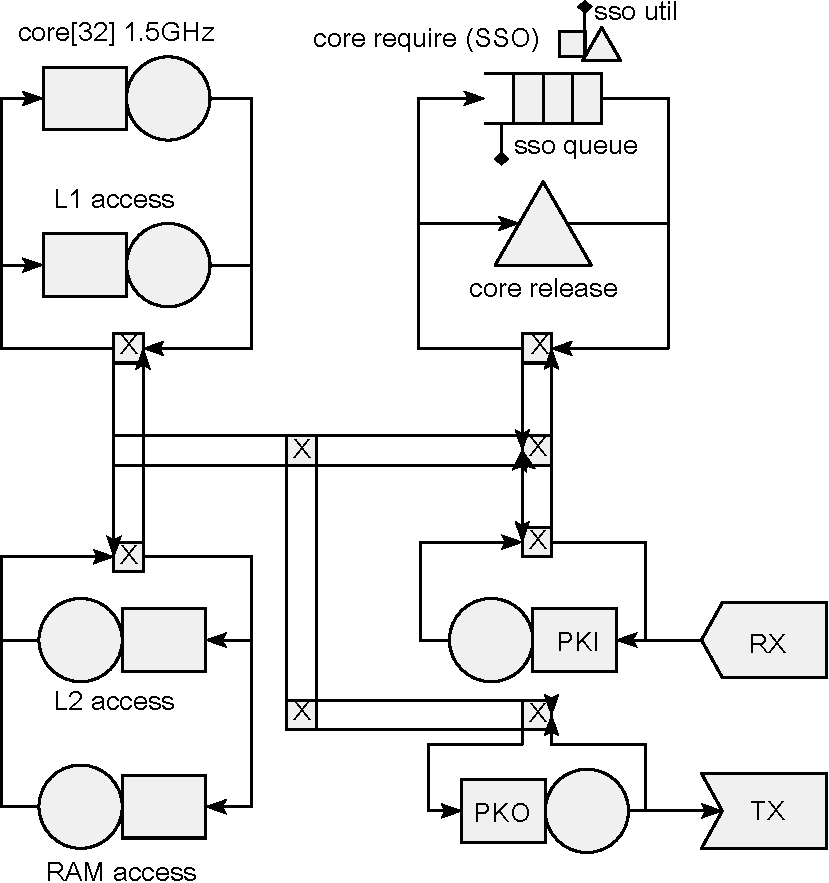
\includegraphics[width=0.6\textwidth]{images/pse-models/experiment-hardware.pdf}
    \caption{Resource provision model (hardware) used in the experiments.}
    \label{fig:experiment-hardware}
  \end{center}
\end{figure}

The scheduler unit uses the custom scheduling functions presented in Section~\ref{sec:scheduler-unit}, enabling the use of atomicity, queue priorities, and coremasks. The core release is a typical release node referring to the scheduler unit.

The same high level software model is used for the both experiments, as seen in the Figures~\ref{fig:exp1-software} and~\ref{fig:exp2-software}. The \emph{Packet Input} and \emph{Packet Output} nodes consume the PKI and PKO units as discussed in Section~\ref{sec:characteristic-measurements}, delaying the packets relative to their size, according to the equation~\ref{eq:1}. The workload and packet process submodels are unique for both experiments.

We gather two different metrics of the system. First, we are interested in the core utilization and queue lengths for each processing step. These are measured by the probes attached to the scheduler unit as shown in hardware model in Figure~\ref{fig:experiment-hardware}. Secondly, we are interested in the packet latencies. They are measured by calculating the time difference between the \emph{out probe} and the \emph{in probe} (Figures~\ref{fig:exp1-software} and~\ref{fig:exp2-software}) for each packet. All the probes write absolute traces of the packets.

\section{Experiment 1: Global Queue Interrelations}
The first experiment consists of two different simulations and measurements. We will first demonstrate a packet processing application, whose throughput is limited due to the bottleneck occurring from a slow atomic processing. The application is then modified, extracting part of the atomic execution object into parallel, thus breaking the bottleneck.

The workload model consists of a single packet stream, which is generated from a two level workload model, presented at the top in Figure~\ref{fig:exp1-software}. The \emph{TRAFFIC GENERATOR} node triggers its child node with interval $RNS\_random\_uniform(5*10^{-5}, 15*10^{-5})$ seconds, and lifetime of 0.05 seconds. The child node creates 512B packets with interval $5.1~*~10^{-8}~* RNS\_random\_lognormal(-10, 0.9)$ seconds for $4*10^{-5}$ seconds.

The two different applications used in the experiment are shown in the software model after the \emph{select app}-node. The lower and upper application are referred as \emph{application 1} and \emph{application 2}, respectively. The application selection is done in the workload model by the \emph{AppId} attribute.

Application 1 consists of two processing steps, both consuming CPU and memory for the range of 5000 clock cycles. The first step consists of parallel, priority 2 queue (A), and the second one is done atomically with priority 1 queue (B). Application 2 is a modified version of the first packet processing application, where the second processing step is split into parallel and atomic steps. The release nodes are omitted from the software model for clarity.

\begin{figure}[]
  \begin{center}
    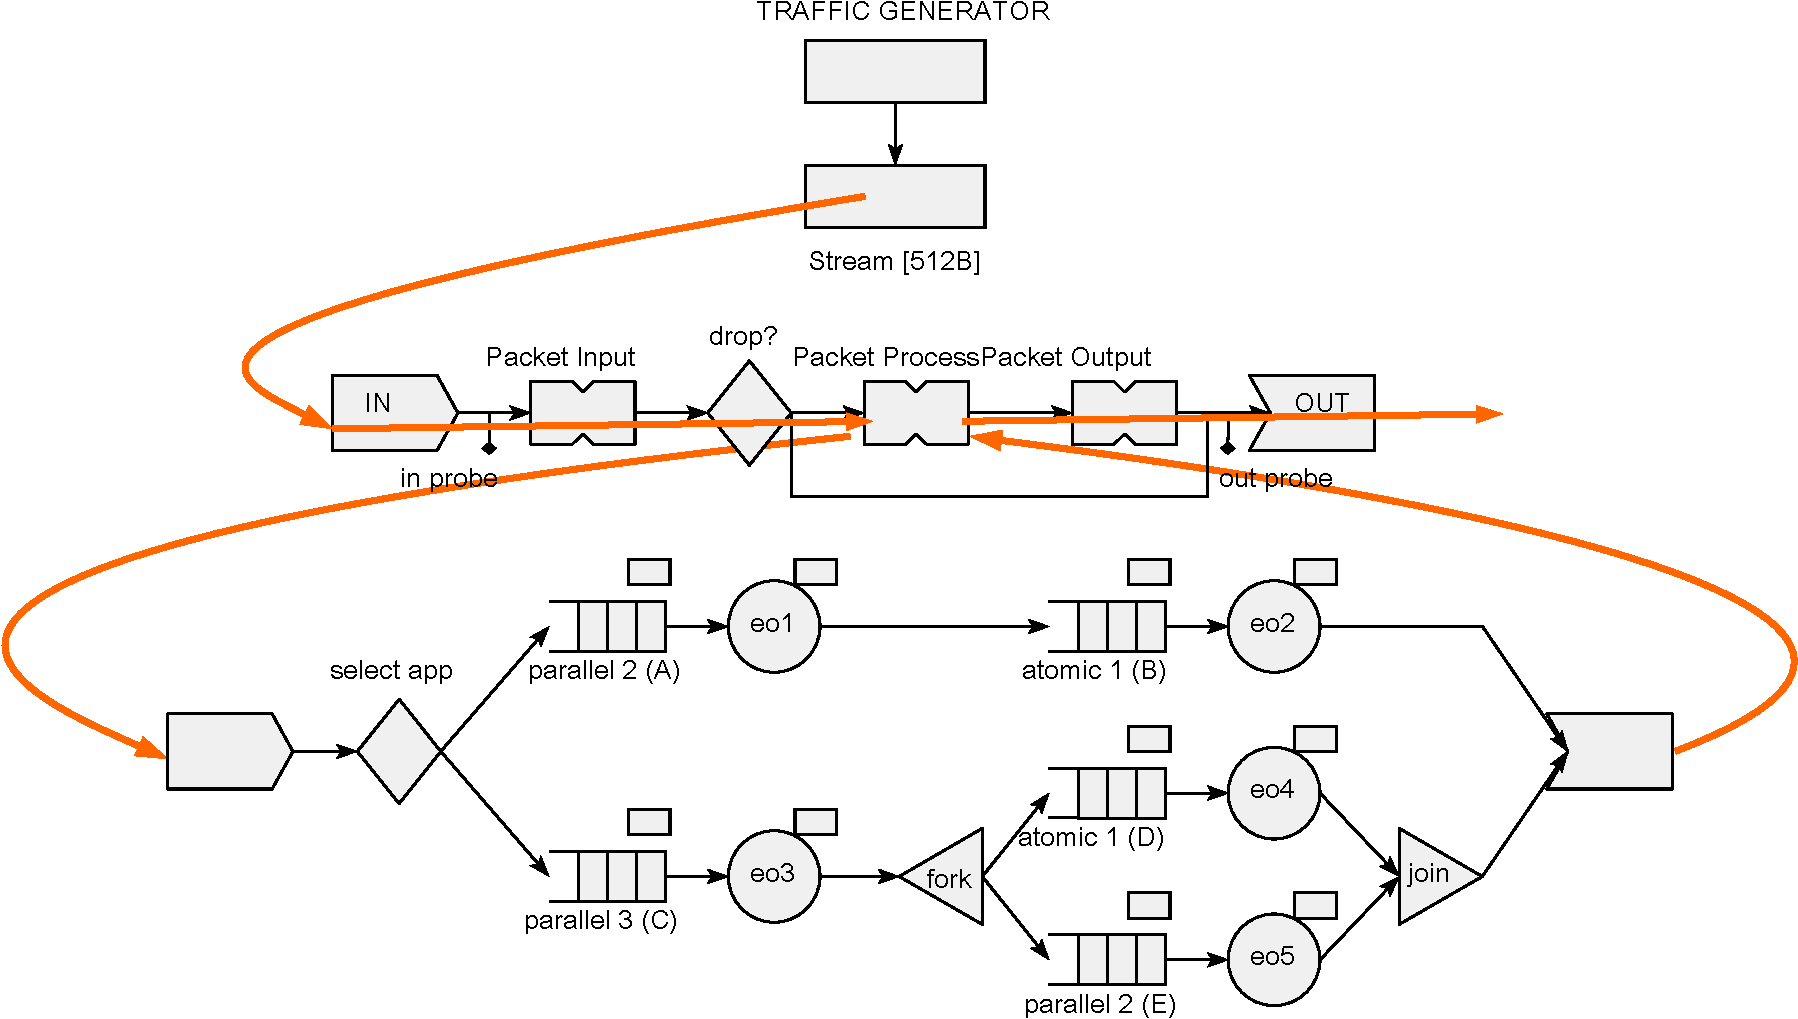
\includegraphics[width=\textwidth]{images/pse-models/exp1-software.pdf}
    \caption{Workload and resource usage (software) models used in the first experiment. The atomic queue in the upper application (application 1) produces a bottleneck to the system. The application 2 below removes this bottleneck by extracting part of the processing into parallel.}
    \label{fig:exp1-software}
  \end{center}
\end{figure}

\subsection{Simulation Measurements}
\label{sec:exp1-simulation-measurements}
The system was simulated using both applications separately, and the data from the probes were post-processed. We grouped the number of tasks in the scheduler/core queue, by the processing step.

Figures~\ref{fig:app1-queue2} and~\ref{fig:app1-latency} present the data from the first simulation using the packet processing application 1. Figure~\ref{fig:app1-queue2} describes the number of tasks in the scheduler/core queue, that are from the atomic resource usage queue, with respect to simulation time. The corresponding graph for the first queue is omitted, as none of that tasks from it end up in the waiting queue. Figure~\ref{fig:app1-latency} presents the latency of each packet through the whole system.

\begin{figure}[]
  \begin{center}
    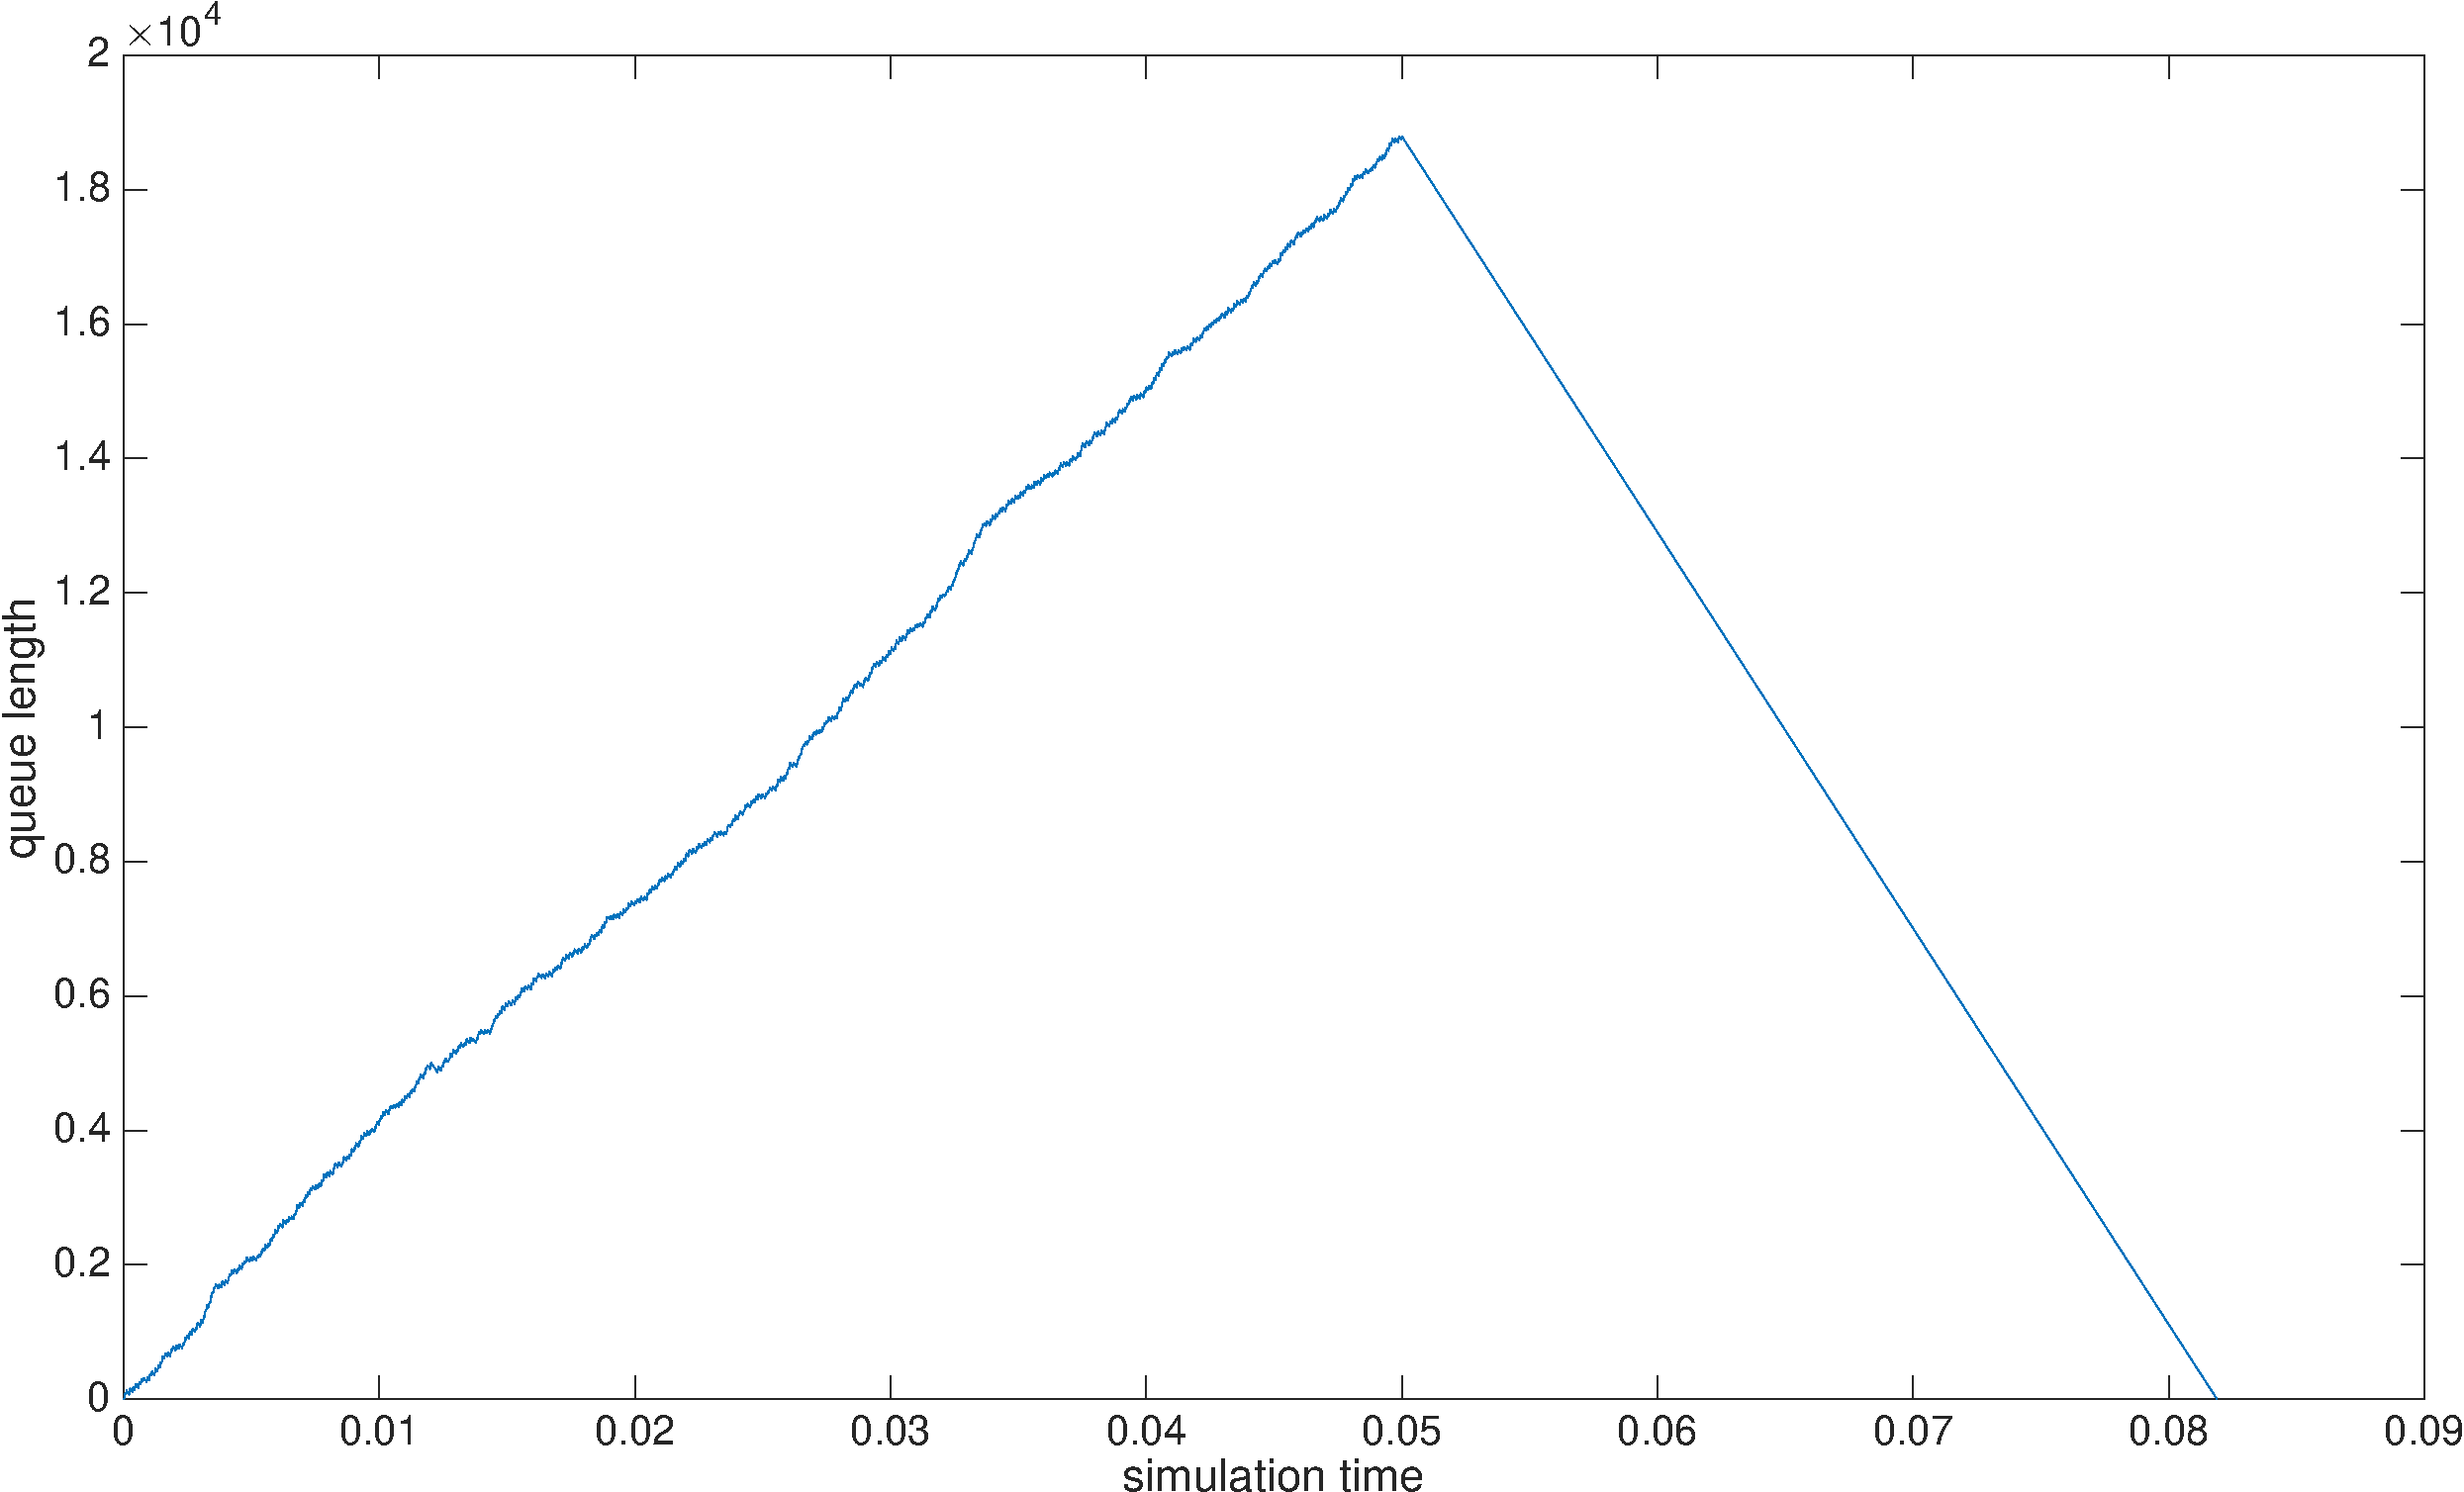
\includegraphics[width=\textwidth]{images/experiment/app1-queue2.pdf}
    \caption{Application 1: The number of tasks in the scheduler/core queue, with respect to simulation time, from the second resource usage queue.}
    \label{fig:app1-queue2}
  \end{center}
\end{figure}

\begin{figure}[]
  \begin{center}
    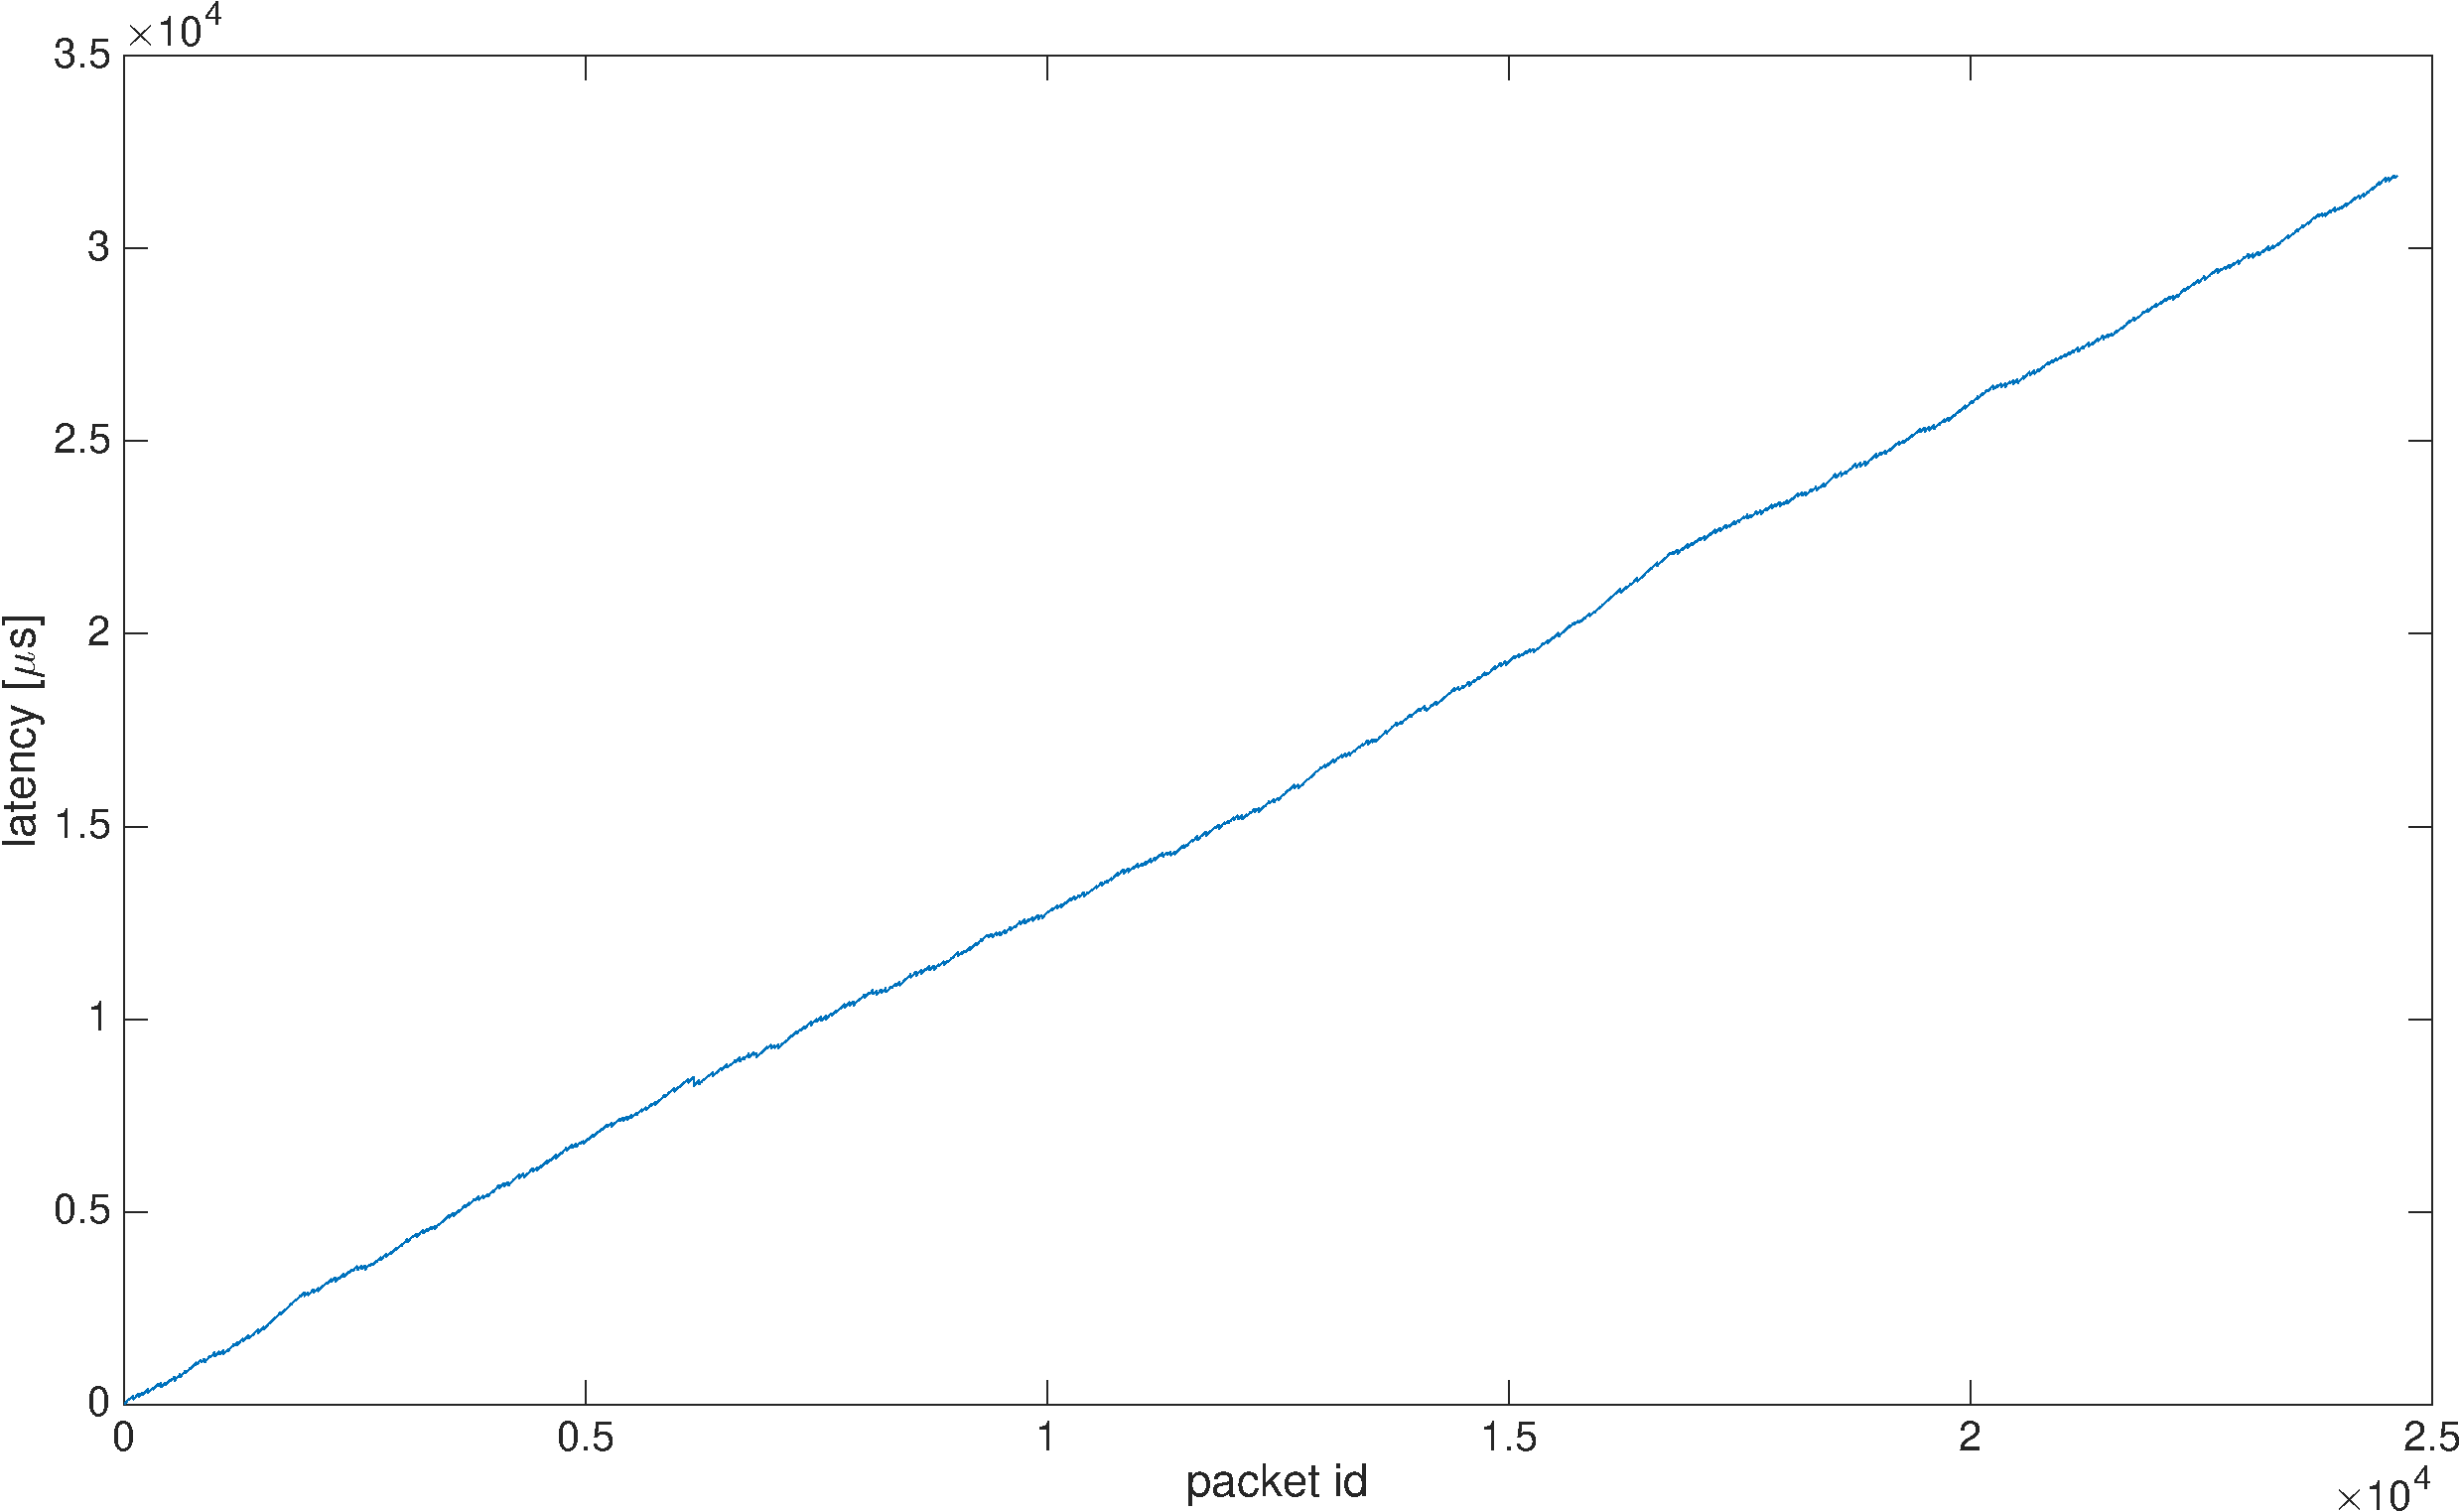
\includegraphics[width=\textwidth]{images/experiment/app1-latency.pdf}
    \caption{Application 1: Latency of the packets through the system.}
    \label{fig:app1-latency}
  \end{center}
\end{figure}

As shown in the Figures, the processing in the second execution object of application 1 is so heavy that the tasks accumulate into the waiting queue, and thus the packet latency keeps growing until the workload ceases.

The second application modifies the system by parallelizing part of the atomic processing. Figures~\ref{fig:app2-queue2} and~\ref{fig:app2-latency} present the data from the second application simulation. Figure~\ref{fig:app2-queue2} shows the number of tasks in the scheduler/core queue, that are from the atomic resource usage queue, with respect to simulation time. Figure~\ref{fig:app2-latency} presents the latency of the packets through the whole system. Neither of the parallel queues have tasks in the waiting queue of the scheduler/core during the simulation.

\begin{figure}[]
  \begin{center}
    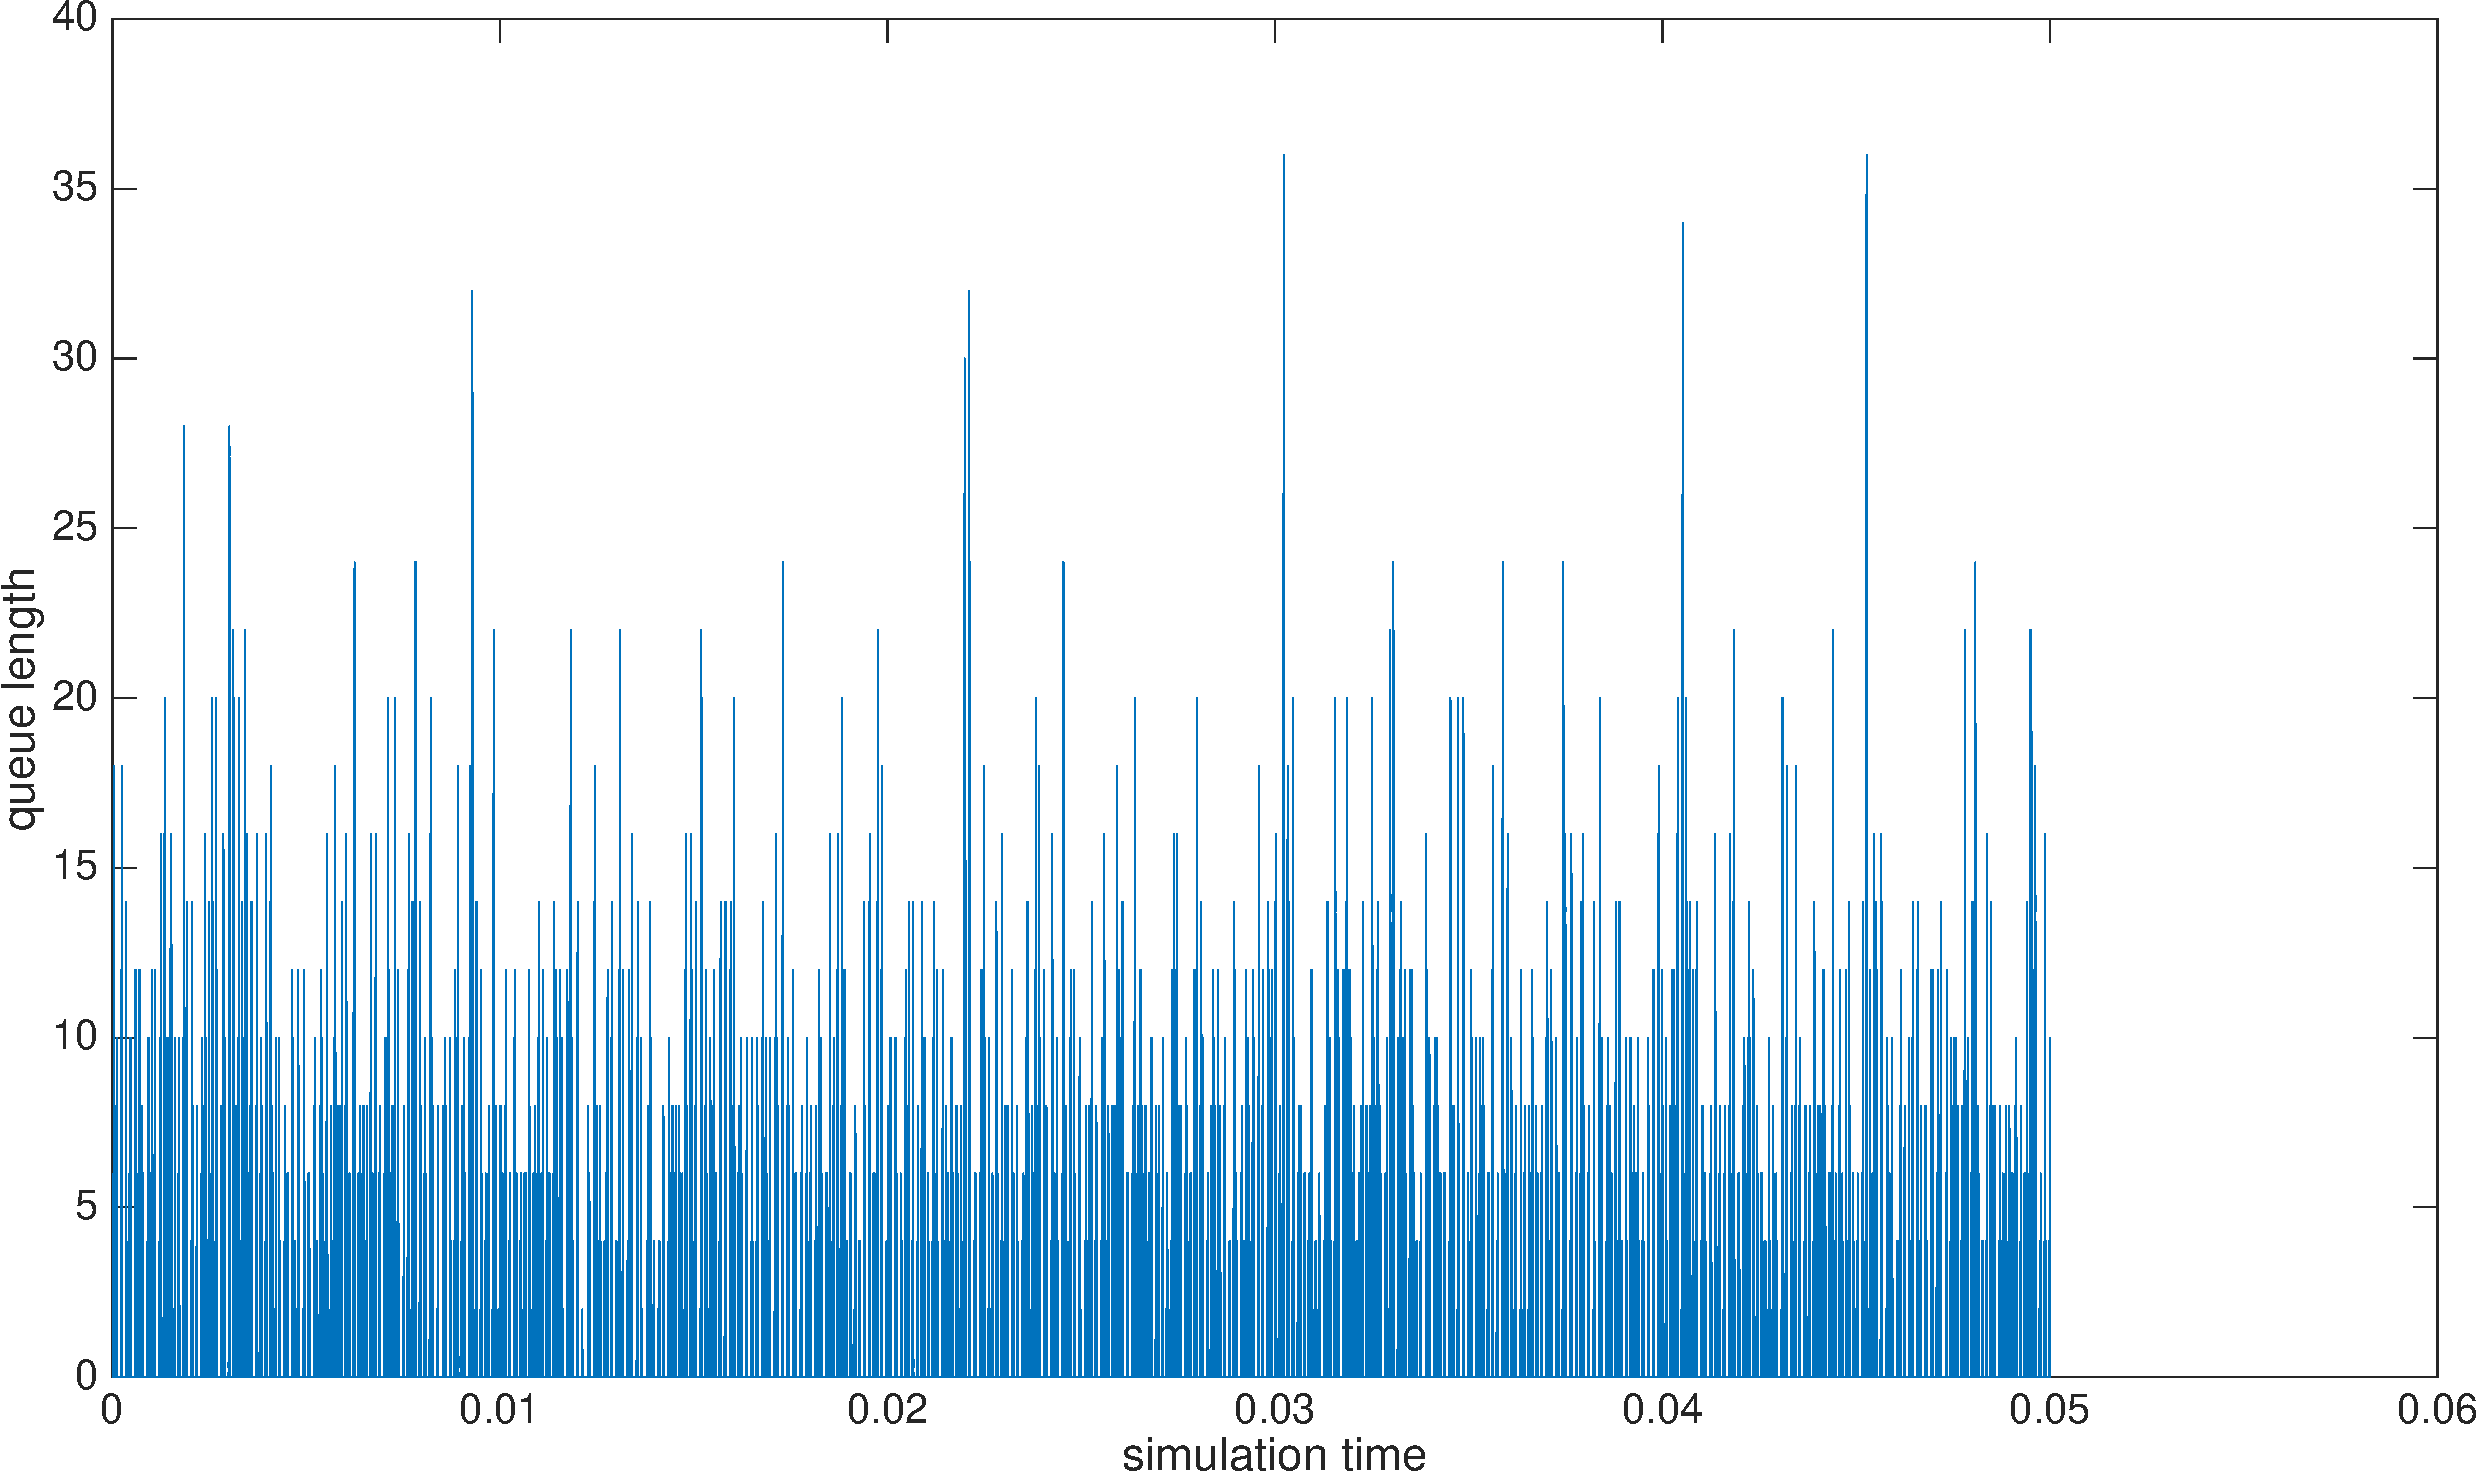
\includegraphics[width=\textwidth]{images/experiment/app2-queue2.pdf}
    \caption{Application 2: The number of tasks in the scheduler/core queue, from the second resource usage queue.}
    \label{fig:app2-queue2}
  \end{center}
\end{figure}

\begin{figure}[]
  \begin{center}
    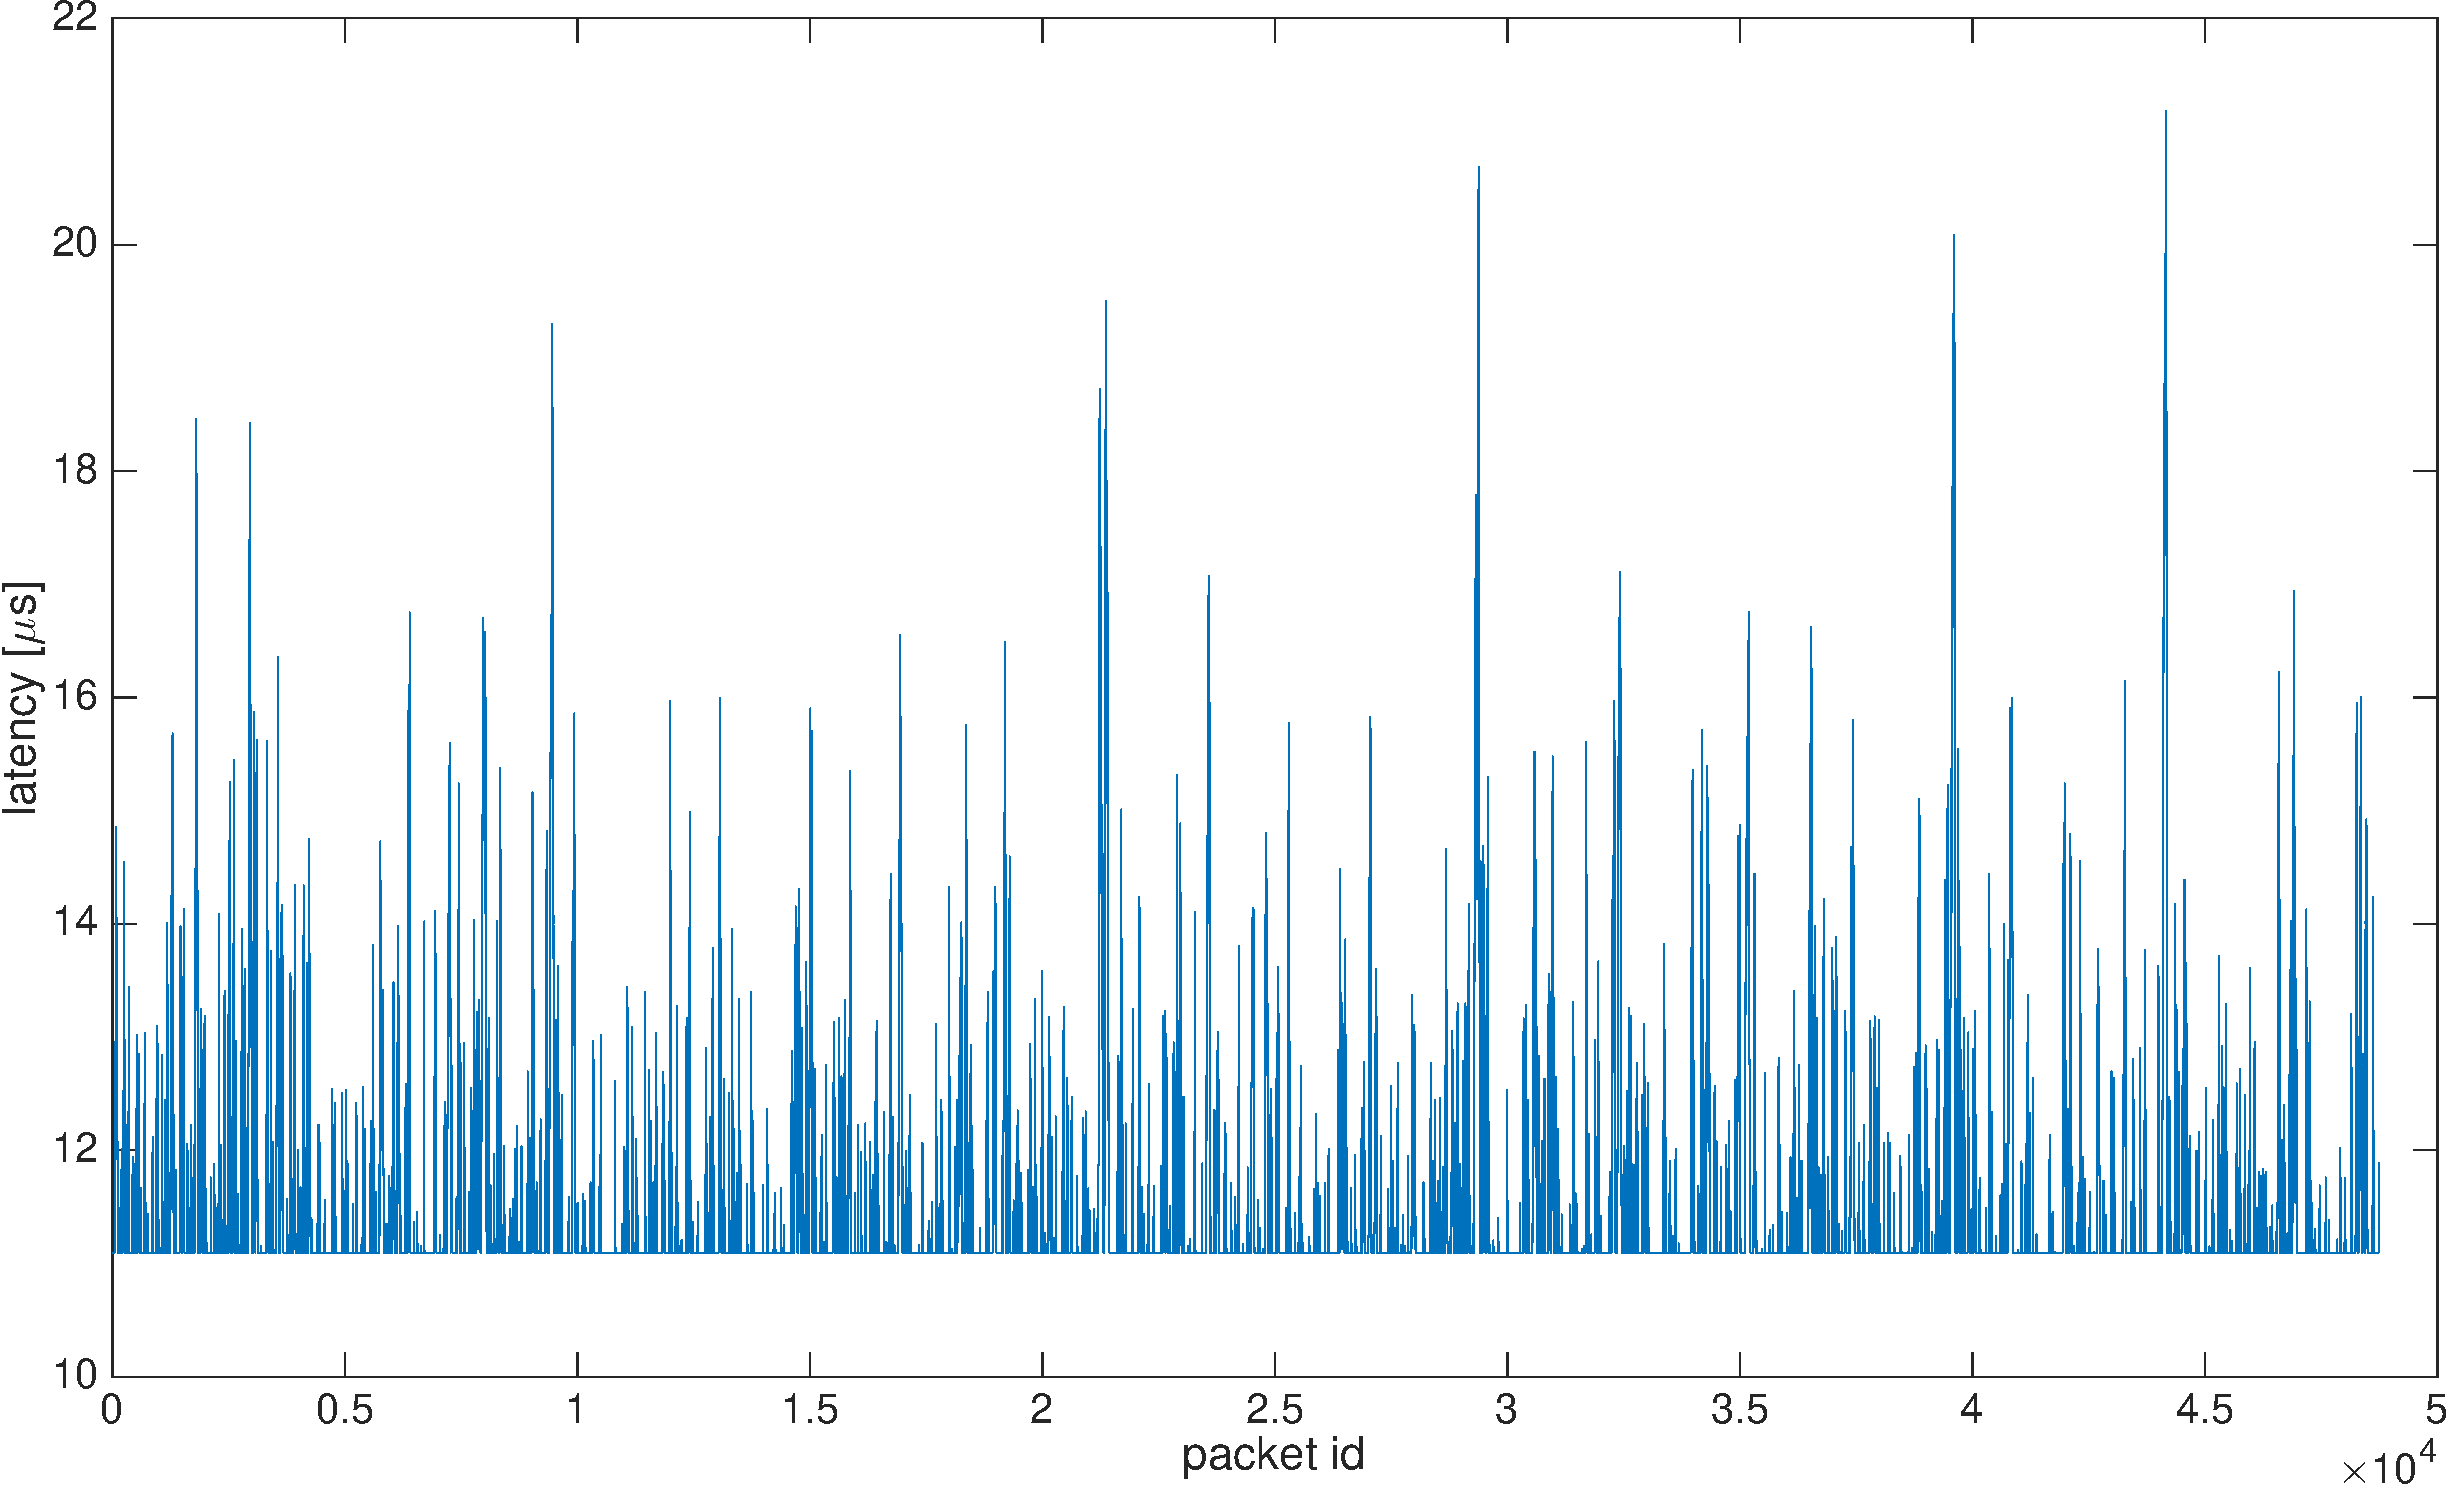
\includegraphics[width=\textwidth]{images/experiment/app2-latency.pdf}
    \caption{Application 2: Latency of the packets through the system.}
    \label{fig:app2-latency}
  \end{center}
\end{figure}

As the shown in the Figures~\ref{fig:app2-queue2} and~\ref{fig:app2-latency}, the latencies of the second application stay within 22$\mu$s, reducing the queue length below 40 over the whole simulation period.

\section{Experiment 2: Queue Coremasks}
% app1 heavy
% app2 light

The second experiment demonstrates the packet flow control via queue coremasks. The experiment consists of two packet flows and dedicated application processing them, as presented in Figure~\ref{fig:exp2-software}. The first packet stream (presented as orange), presents a higher OSI-level application data, such as video stream, which is processed on a heavy execution object. The second stream (presented as blue), on the other hand, consists of packets whose processing is done on fast processing application with strict latency requirements.

The \emph{TRAFFIC GENERATOR} node triggers its child nodes with interval $RNS\_random\_uniform(5*10^{-5}, 15*10^{-5})$ seconds, and lifetime of 0.05 seconds. \emph{Stream 1} and \emph{Stream 2} create 512B packets with interval $6.1*10^{-7}~*~RNS\_lognormal(-10, 0.9)$ and $10^{-6}~*~RNS\_lognormal(5, 10)$ seconds for $4*10^{-5}$ and $10^{-5}$ seconds, respectively. The heavy application consumes the CPU and memory for a total of about 50000 cycles per 512B packet, while the light application packets are processed for tenth of that, in 4500 cycles.

We will again perform two different simulations and measurements. The first one is carried out by allowing the heavy application to be processed on all the 32 processing cores. Despite the light flow being processed on higher priority queue, the processing of the heavy flow has an effect to the worst-case latency of the light flow packets. This happens due to the run-to-completion model of the cores, where light flow packets may have to queue for a core while the heavy tasks finish. In the second simulation, the heavy application processing is limited to 30 cores, dedicating two cores for the light application.

\begin{figure}[]
  \begin{center}
    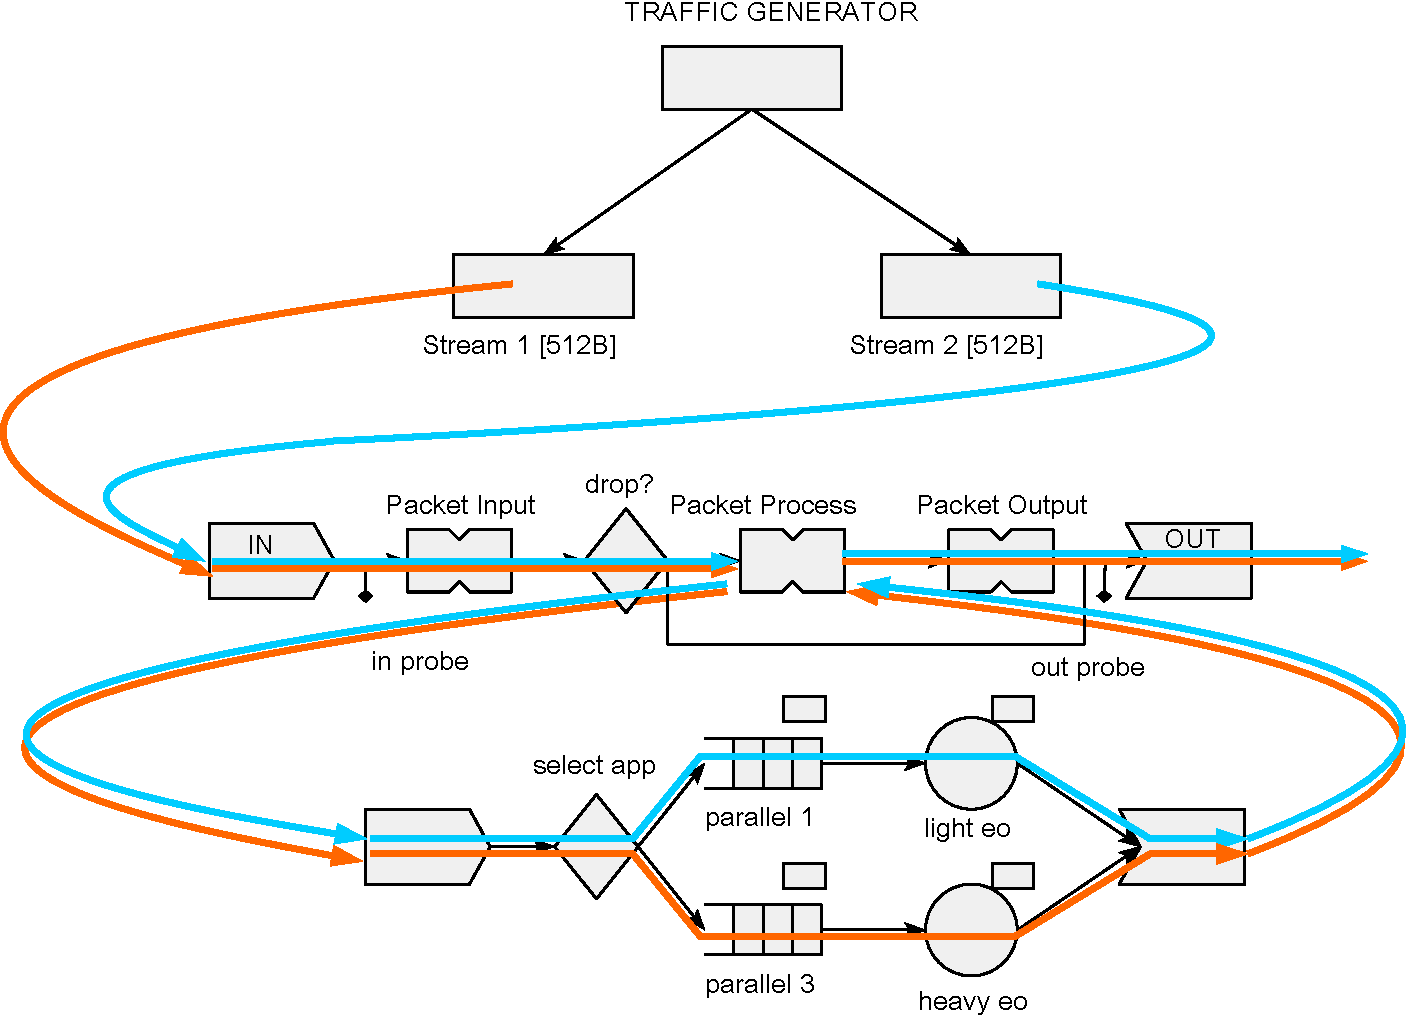
\includegraphics[width=\textwidth]{images/pse-models/exp2-software.pdf}
    \caption{An overview of the workload and software  models used in the experiment 2. The orange and blue paths present the paths of the packets through the system. Each of the flows has its own packet processing application.}
    \label{fig:exp2-software}
  \end{center}
\end{figure}

\subsection{Simulation Measurements}
\label{sec:exp2-simulation-measurements}

The system was simulated with and without the limited coremask on the heavy application processing cores. The data from the probes were then post-processed. Figures~\ref{fig:exp2-app1-no-coremask-latency} and~\ref{fig:exp2-app2-no-coremask-latency} present the data from the simulation without coremask, for the heavy and light flow, respectively. The latency of the heavy flow packets is between 80$\mu$s and 340$\mu$s throughout the simulation. The throughput of the heavy application is 0.214GBps.

\begin{figure}[]
  \begin{center}
    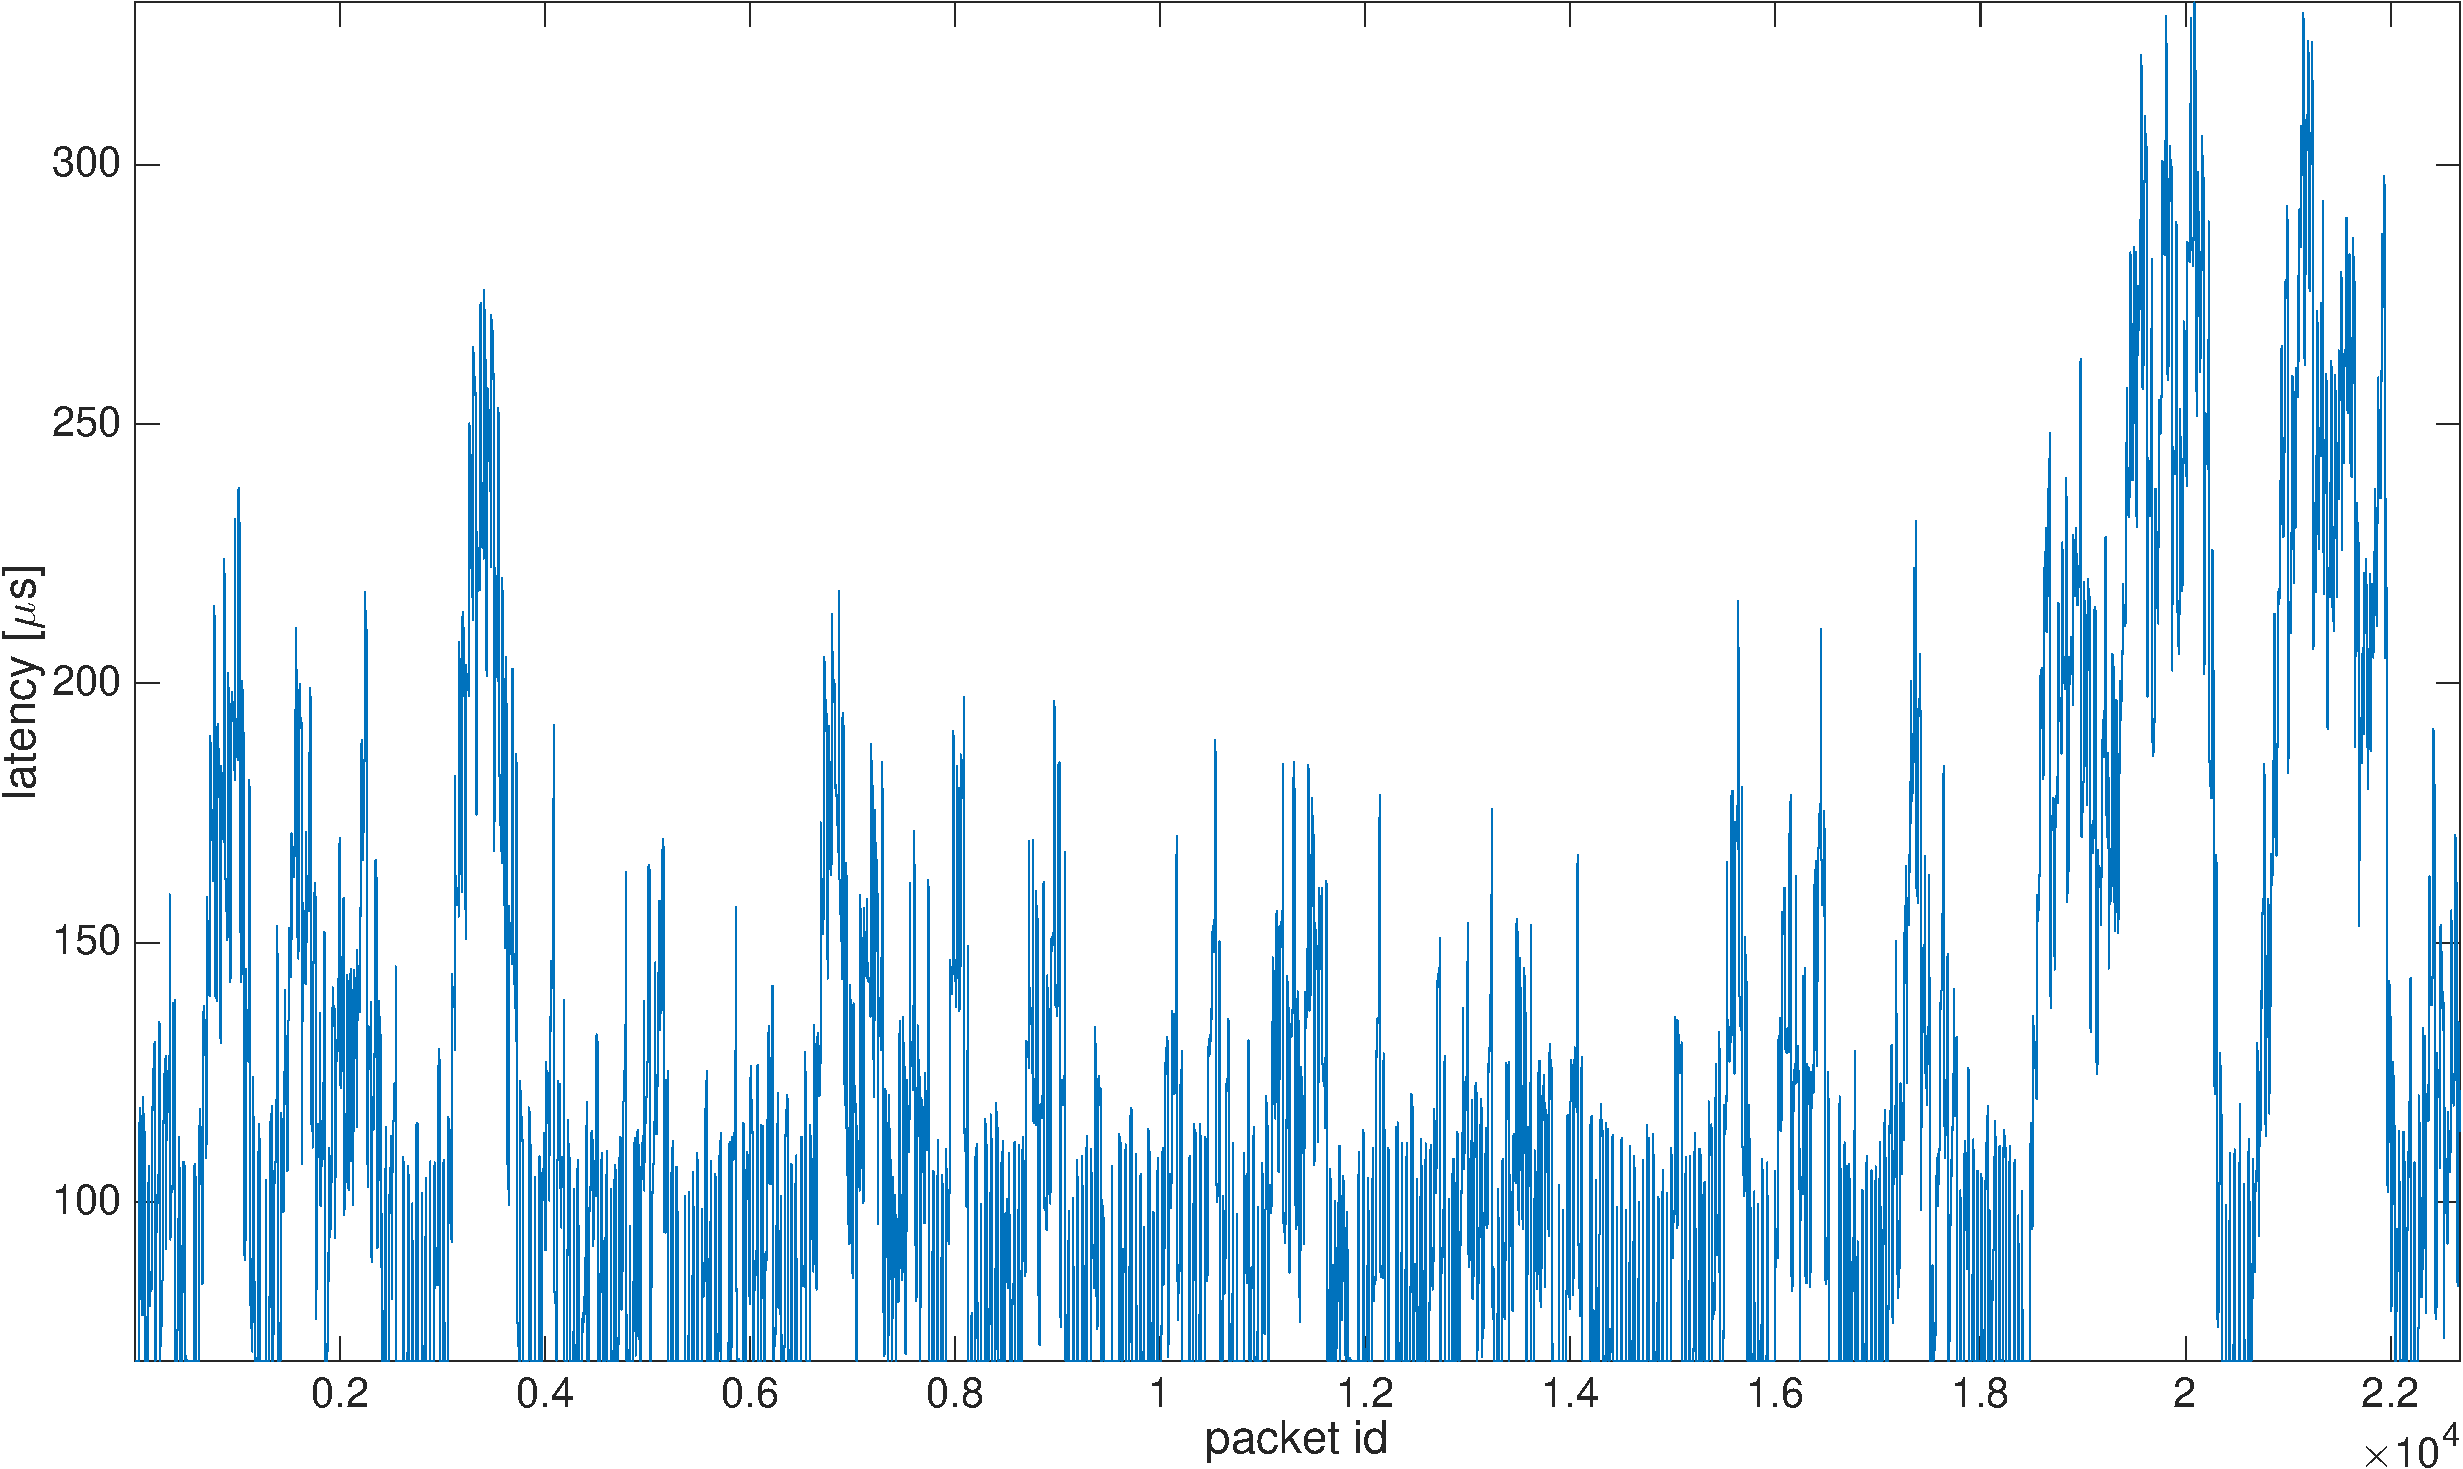
\includegraphics[width=\textwidth]{images/experiment/exp2-app1-no-coremask-latency.pdf}
    \caption{Latencies of the heavy flow packets, without coremask.}
    \label{fig:exp2-app1-no-coremask-latency}
  \end{center}
\end{figure}

\begin{figure}[]
  \begin{center}
    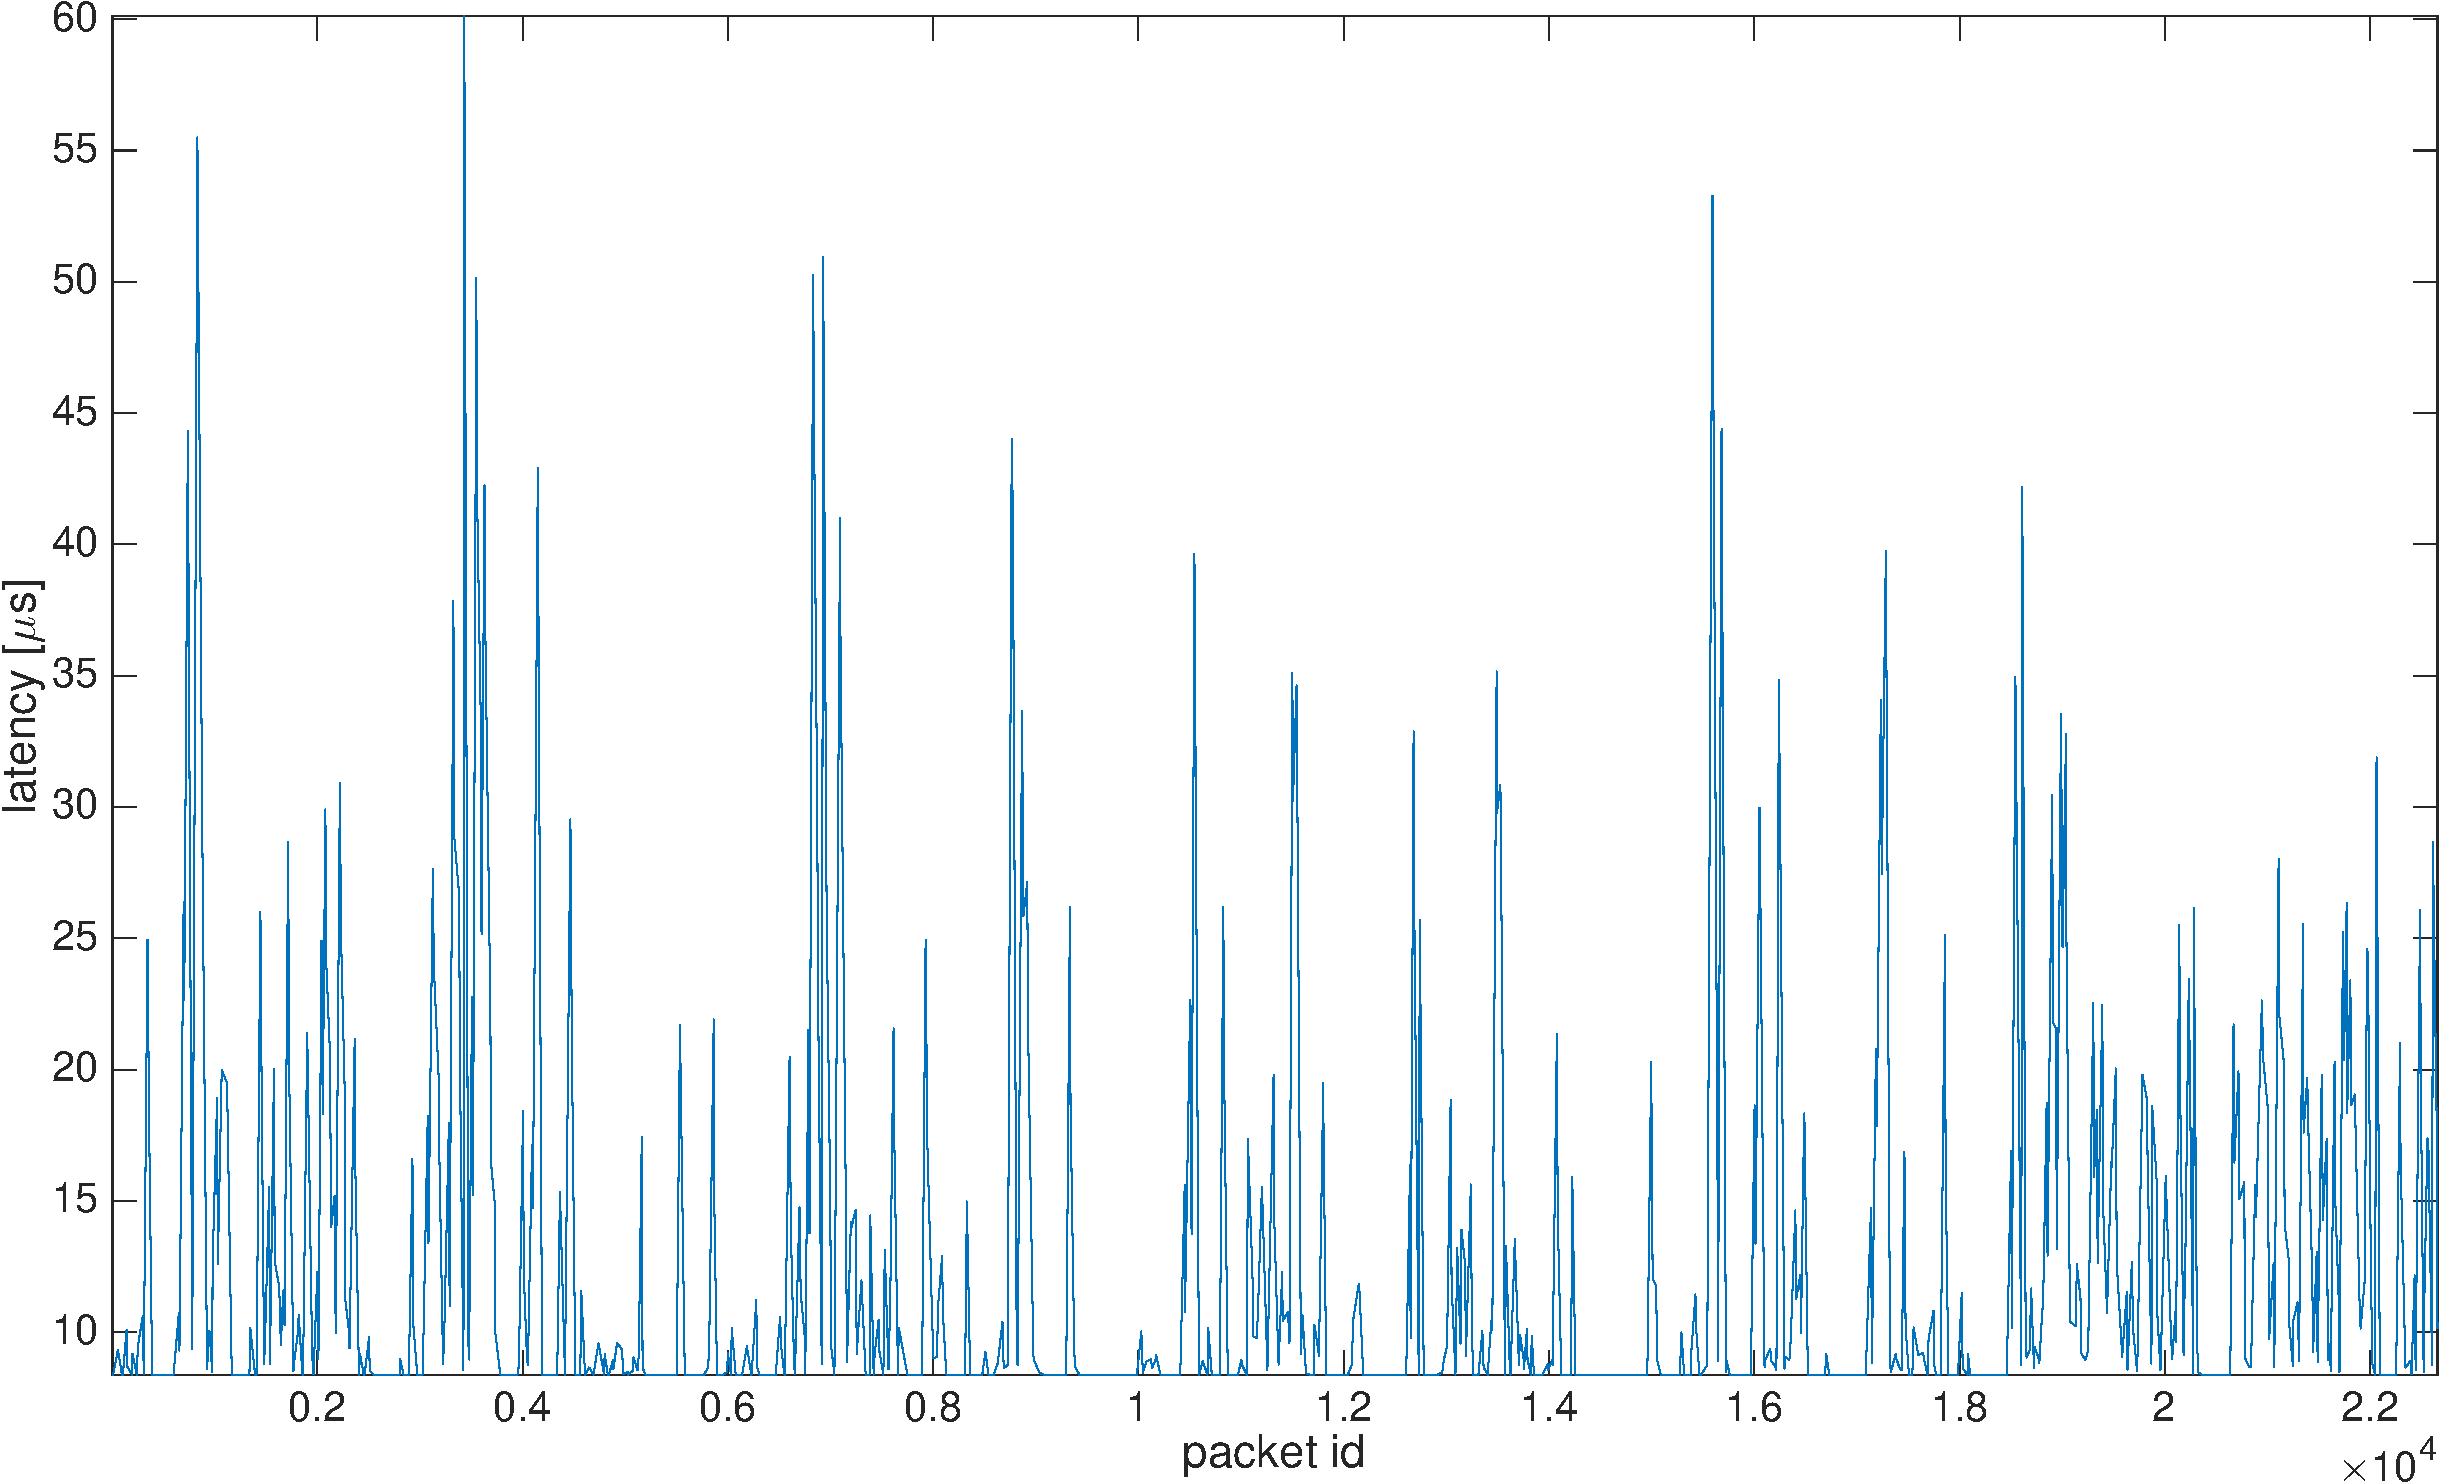
\includegraphics[width=\textwidth]{images/experiment/exp2-app2-no-coremask-latency.pdf}
    \caption{Latencies of the light flow packets, without coremask. The worst-case latencies are almost ten-fold compared to the best-case.}
    \label{fig:exp2-app2-no-coremask-latency}
  \end{center}
\end{figure}

In the second simulation, we use a modified coremask for the heavy application, i.e. dedicating one of the cores for the light application processing. The resulting latencies of the heavy and light flow are presented in Figures~\ref{fig:exp2-app1-is-coremask-latency} and~\ref{fig:exp2-app2-is-coremask-latency}, respectively. The light flow's worst-case packet latencies stay below 12$\mu$s. The throughput of the heavy application is 0.212GBps.

\begin{figure}[]
  \begin{center}
    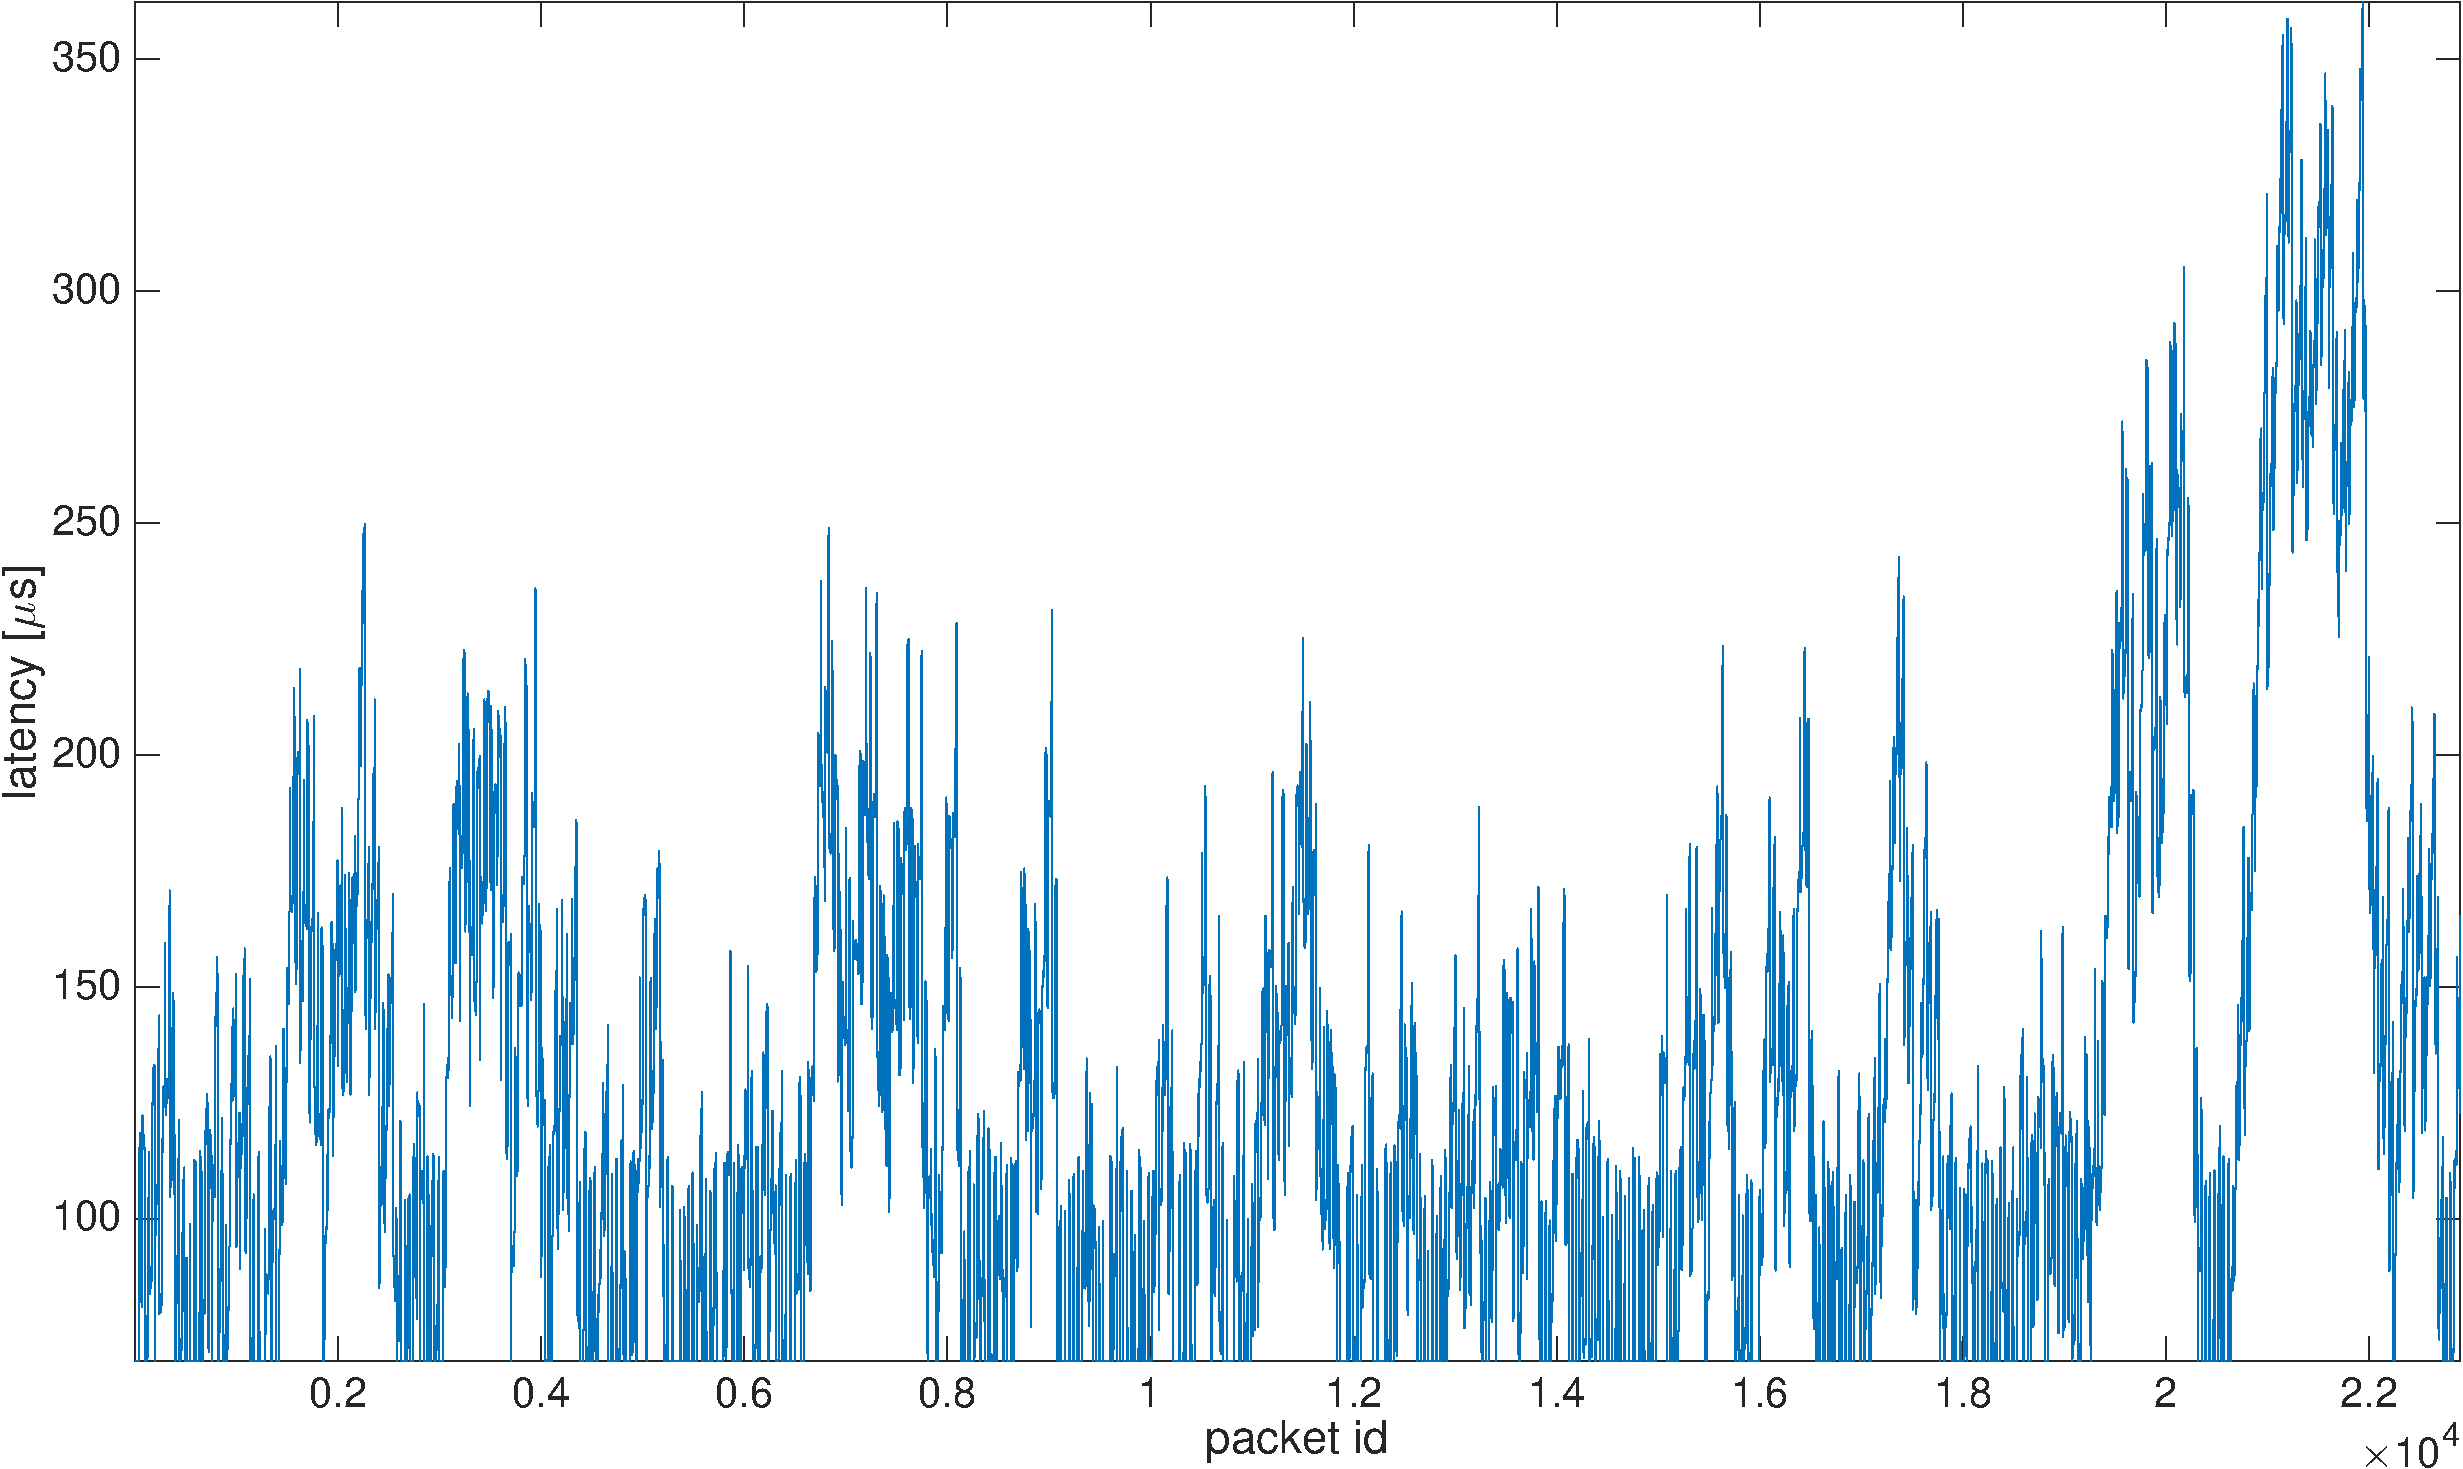
\includegraphics[width=\textwidth]{images/experiment/exp2-app1-is-coremask-latency.pdf}
    \caption{Latencies of the heavy flow packets. One of the cores is dedicated for the light flow.}
    \label{fig:exp2-app1-is-coremask-latency}
  \end{center}
\end{figure}

\begin{figure}[]
  \begin{center}
    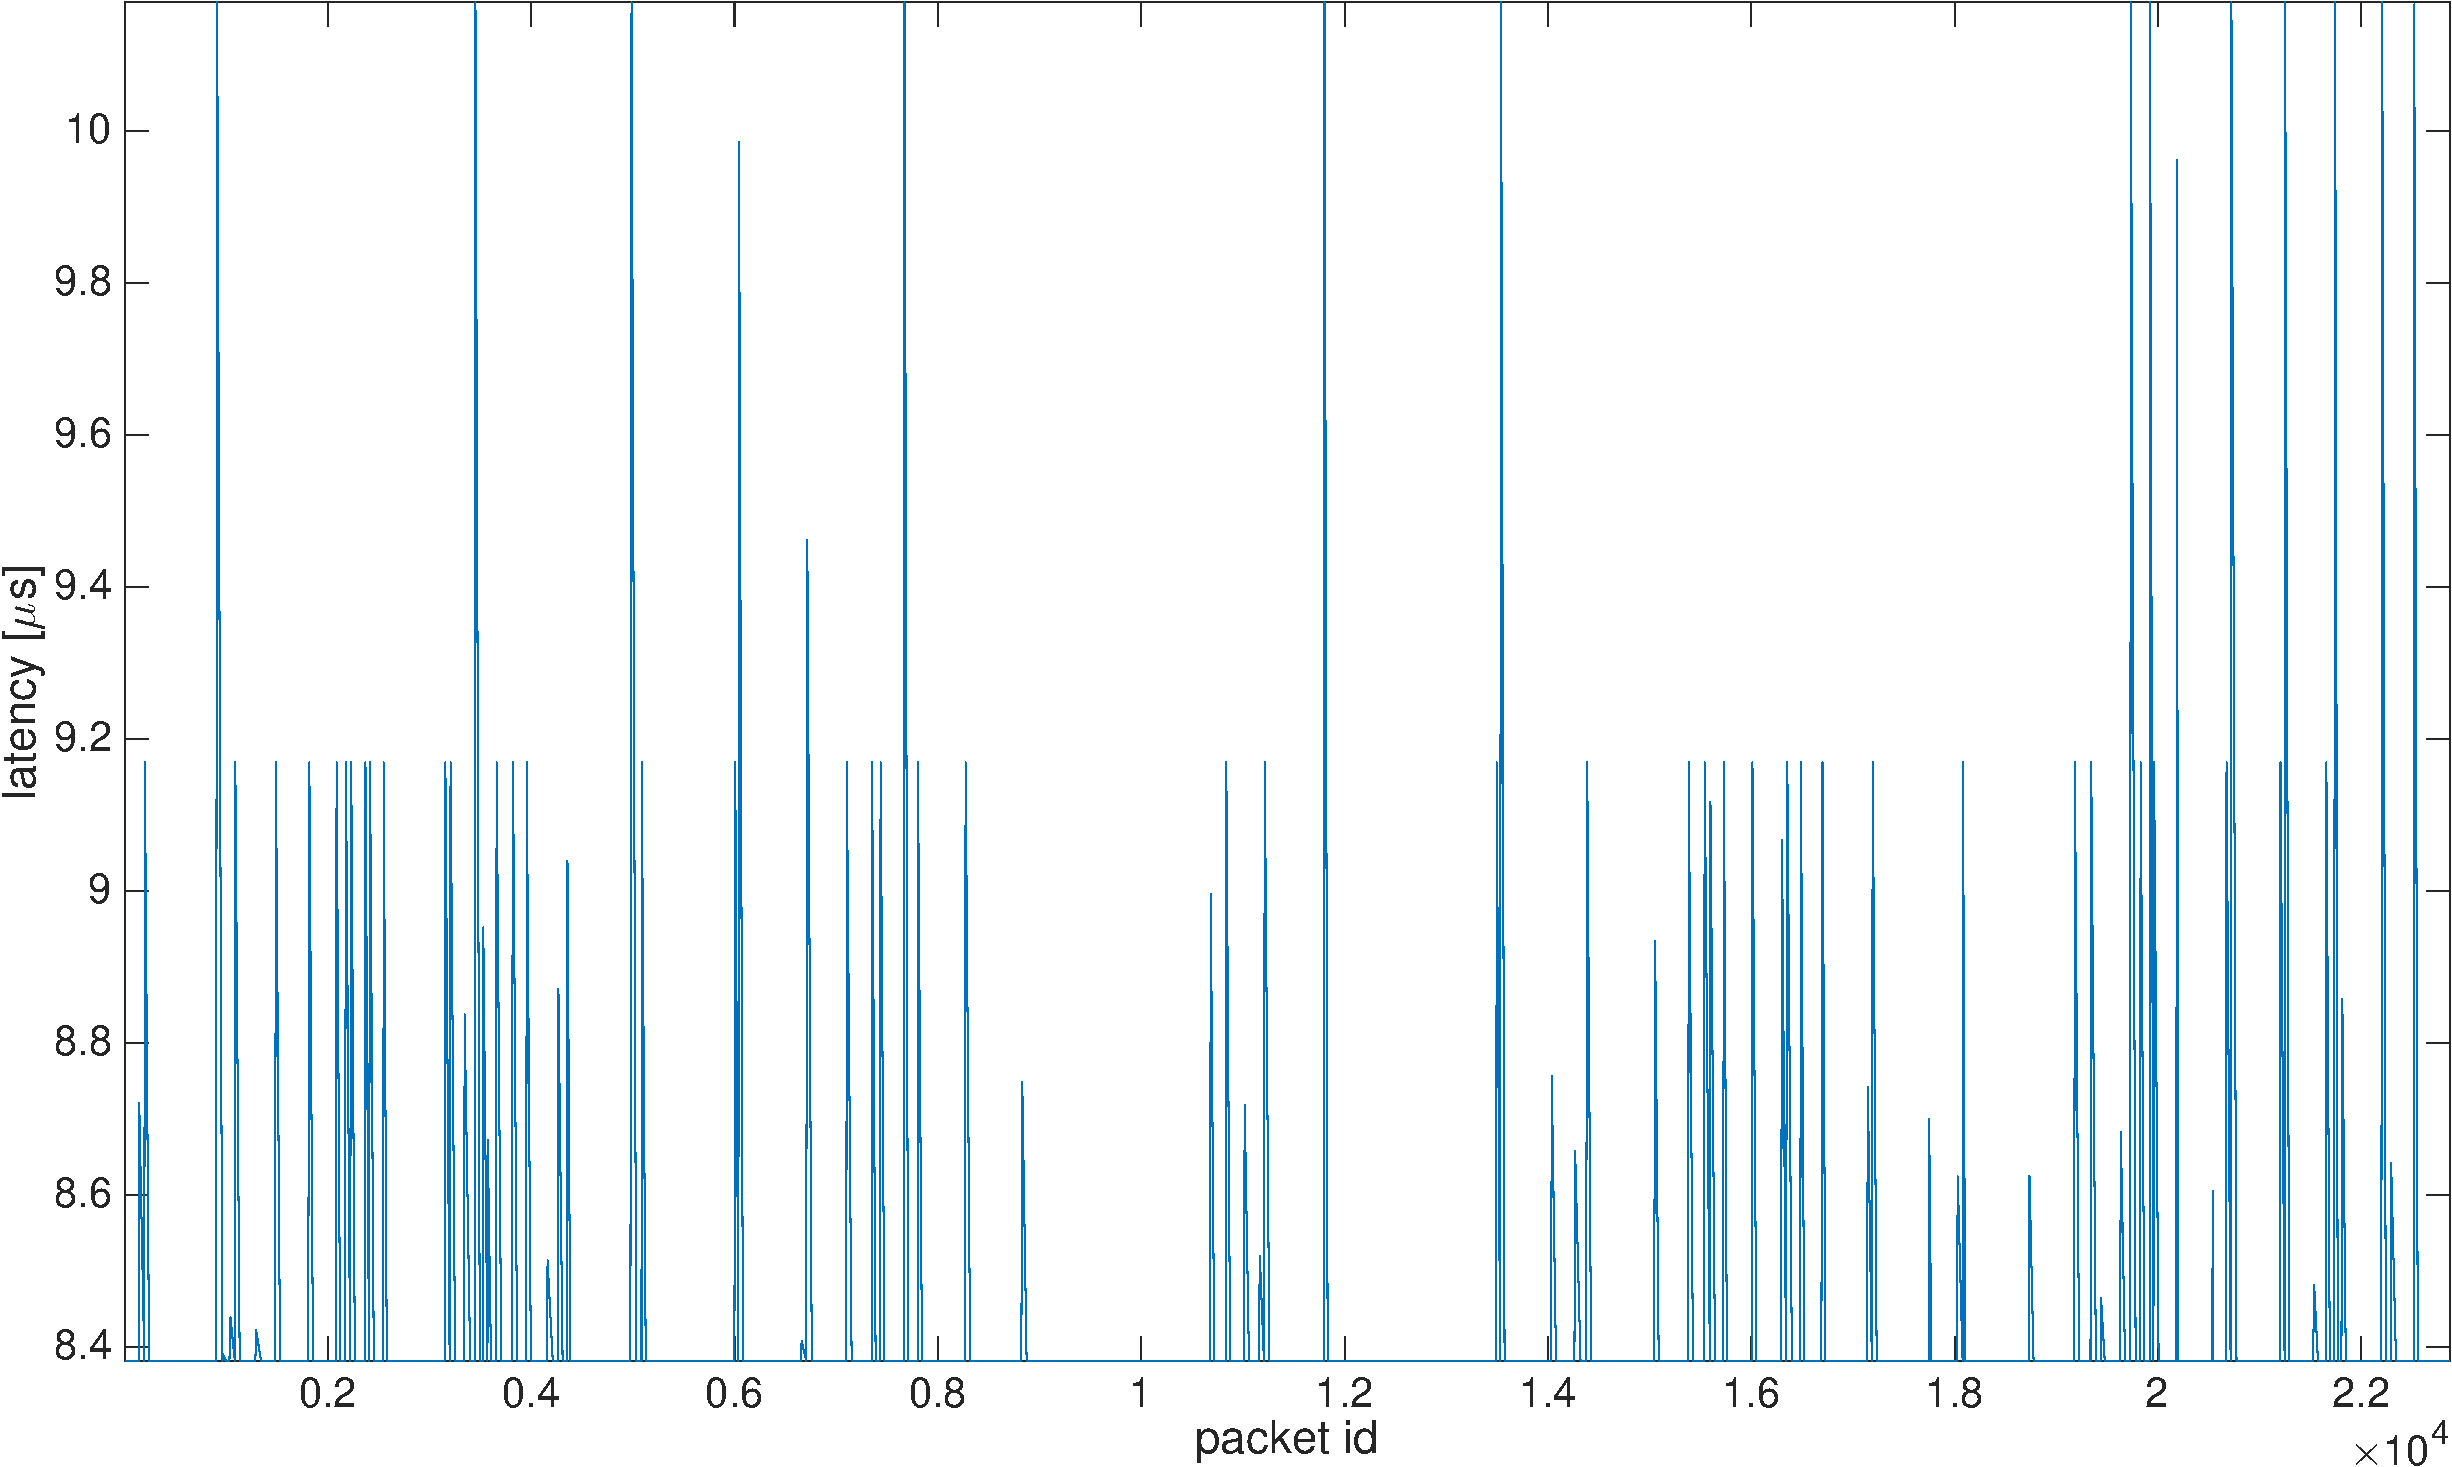
\includegraphics[width=\textwidth]{images/experiment/exp2-app2-is-coremask-latency.pdf}
    \caption{Latencies of the light flow packets. One of the cores is dedicated for the light flow. The worst-case latencies are less than 50\% higher than of the best-case.}
    \label{fig:exp2-app2-is-coremask-latency}
  \end{center}
\end{figure}

\section{Experiment Analysis}

The experiments present a proof of concept of the implemented PSE's plugin code mechanism and the model of the reference NPU. In both experiments, the model acts as expected.

The first experiment presents the use the global queue information to control the resource provision based on global queue priorities and disciplines. As seen in the Figures~\ref{fig:app1-queue2} and~\ref{fig:app1-latency}, the second processing step produces a bottleneck to the system. This happens due to the atomicity of the second processing queue, forcing heavy processing of the packets one at a time. By dividing the atomic processing step into a smaller atomic part and larger parallel part, the latency of the system should be reduced, as the atomic part of the processing can be done faster, and the cores can fully be utilized by the heavier parallel part of the second processing step. The measurements results of the second application, as shown in the Figures~\ref{fig:app2-queue2} and~\ref{fig:app2-latency}, validate this behavior.

The second experiment presents the use of queue coremasks, to control the use of specific hardware resources, through the software model. As shown in the Figure~\ref{fig:exp2-app2-no-coremask-latency}, without limiting the coremask, the light flow packets can be processed in 8$\mu$s at best. However, in the worst-case, when all the cores are processing heavy flow packets, the light flow packet latency is almost ten-fold compared to the best-case latency, 61$\mu$s. By dedicating a processing core for the light flow, we sacrifice the throughput of the heavy flow in order to reduce the worst-case latency of the light flow. As shown in the Figure~\ref{fig:exp2-app2-is-coremask-latency}, changing the coremask in the software model removes the bottleneck from the system. The light flow's worst-case packet latencies can be reduced to less than 50\% higher than of the best-case, while the heavy flow's throughput drops only 2\% compared to the non-coremask processing.

The experiments also highlight the PSE's ability to decouple the hardware and software model. All the changes in the experiment applications can be done easily through the four software model files. Once the resource provision model and the high level resource usage models are built, the application developers can prototype the system with by modifying only the software and workload parts of the model corresponding the real software applications written in task-based programming models, such as Open Event-Machine. At the same time, the hardware developers can work on the model parts corresponding to the real hardware.

According to the experiment results, the PSE's resource network concept, extended with user-defined queue disciplines, seems to be provide the desired flexibility, both in the abstraction level and the modularity, for modeling complex hardware and software co-scheduled manycore systems, such as the reference network processing unit. More importantly, the plugin code mechanism extends to any resource network based simulation task, providing flexibility, hopefully allowing even more complex systems to be modeled.

\section{Discussion}

\subsection{Challenges}
Performance analysis of packet processing systems involves various challenges. Our work began with the instrumentation of an example packet processing system, but due to the hardware difficulties, we chose to proceed with modeling and simulation methods. The tool, Performance Simulation Environment, used for the study was chosen mainly because of our previous experience with it. The modeling work begins with the proper understanding the different components, such as the hardware, software, and workload of the system under study.

Understanding typical MPSoC based packet processing systems is difficult, due to the architectural heterogeneity, complexity, and non-deterministic behavior. Our study focused on the packet processing system's hardware packet scheduling unit, and the ability to abstract hardware on Open Event-Machine type parallel programming frameworks. We also executed various measurement experiments to gather more detailed characteristics of the hardware memory and ingress- and egress unit behavior. Instrumentation faces the same challenges as any other parallel application development.

Different parallel programming frameworks are used to abstract the hardware from the software application development. To understand the actual applications' effect on the packet processing systems, the underlying runtime frameworks must also be understood. In our work, one of the challenges was to understand the queue based Open Event-Machine implementation, and especially the global scheduler functionality and implementation on different platforms. Also, the actual packet processing functions needed to be understood, in order to create realistic application models.

Hardware system models are difficult to simulate on software; efficient simulation of inherently parallel hardware models requires non-trivial parallelization of the simulator, which has been widely studied research topic for decades. Finding appropriate model abstraction level is essential. On one hand, abstraction level affects the simulation execution time and accuracy of the results. Too detailed models are intractable and require time consuming simulations, while too high-level abstractions hide the sought characteristics of the system, resulting in inadequate results. On the other, it affects the complexity of model
construction and reusability. Higher abstraction levels are used more and more often, as the systems under study are becoming more complex.

\subsection{Discoveries}
In this thesis, we created a model of an MPSoC based packet processing system, running Open Event-Machine type task-parallel packet processing applications on dynamic workloads. The goal of Open Event-Machine is to decouple the hardware and software from each other, and further enable code and performance portability between different systems.

By the implemented user-definable queue disciplines, Performance Simulation Environment (PSE), enables flexible adjustment of modeling abstraction levels. We chose to focus on the hardware packet scheduler unit of the system, and modeled it behavior on a level that enables performance analysis of Open Event-Machine applications on dynamic workloads. The chosen abstraction level hides the details of hardware level memory behavior, but still provides accurate details of Open Event-Machine's software level queues.

The abstraction level, naturally, limits the parallelization possibilities of the underlying simulator engine. When the functionality of the hardware scheduler is modeled, even on high abstraction level as done in our work, the modeling of the hardware parallelism on software eliminates the simulation performance. Also, the use of interrelated global queues increases the data dependencies between the simulation execution, resulting in difficulties in the parallel simulation execution. The problem is common when simulating hardware on software. In our experiments, the simulation performance suffered mostly due to the custom select and reserve functions. The choice to model Open Event-Machine's queue system accurately was intentional, despite its obvious effect on simulation performance.

As our experiments demonstrate, the resource network paradigm extended with custom queuing disciplines and support for modeling task parallelism, is adequate tool for performance analysis of network processing systems, running Open Event-Machine based task-parallel applications on dynamic workloads. PSE separates the workload, software, and hardware models, highlighting the ability to decouple the different functional parts of the system, and enabling modularization and further model reuse.

\subsection{Future Work}
There exist several directions for future research around the topic of this thesis. As we have shown in this work, the resource network methodology, extended with user-definable queue disciplines and support for modeling parallel systems, can be used to model more modern MPSoC based network processing units. The user-defined queue disciplines provide desired flexibility to the PSE's modeling and simulation abstraction level. However, in order to meet the modeling and simulation requirements of larger systems, such as full scale datacenter networks or complex IoT applications, PSE needs to be further developed.

Simulation of large-scale models faces the same challenges as any large scale application. Due to the growing memory and computing resources requirements, the resource usage of PSE needs to be improved.

% One way of improving the simulation efficiency, is to develop the threads executing tasks and the data structures used in the simulation runtime. The threads are fairly heavy structures to handle the tasks, in the context of large-scale simulations. These could, for example, be replaced with similar structures as Akka frameworks' actors. Some of the data structures used in the simulation are dependent on the modeler's choice of the scheduling functions, thus resulting in a tradeoff between the general but less efficient memory structures and the ease of modeling.

Despite the more efficient data structures and single threaded execution, simulator software faces the same problems as any other computer software: efficient scaling requires parallelization of the software. Parallelization of discrete-event simulator software is a wide research topic itself, and faces multiple challenges, not only the ones faced with parallelization in general, but also the simulators' nature makes the problem non-trivial. The parallelization of PSE could be done in several ways. With the current implementation of the PSE, the conservative parallel simulation (the simulation threads advance conservatively) approach seems to be most viable solution. However, to enable more advanced parallelization methods, e.g. variations of optimistic and conservative approaches, parts of the simulator core needs to be rewritten, as the current version of PSE does not support any history of the simulation.

Another future research topic around resource networks is the support for virtualization. Virtualization is an important topic in today's computing, and for example large-scale cloud- and fog datacenters are contingent on the efficient virtualization methods. Performance analysis methods need to adapt to support the needs to further understand these systems. A natural way to model virtualization with resource network concept, would be to add a new virtualization model layer between the resource utilization and resources provision models.

%%% Local Variables:
%%% mode: latex
%%% TeX-master: "thesis-hartikainen"
%%% End:
